% !TeX engine = xelatex
% !TeX spellcheck = en-US
% adjust to 16:9 for displays. you can just use \documentclass[handout]{ctexbeamer} for notes

\documentclass[aspectratio=169]{beamer}
\usepackage{booktabs}
\usepackage{svg}
\usepackage{fontawesome}
\usepackage[style=authortitle-comp,backend=bibtex]{biblatex}
\usecolortheme{seagull}
\setbeamertemplate{sidebar right}{}
\setbeamertemplate{footline}{%
	\hfill\usebeamertemplate***{navigation symbols}
    \hspace{1cm}\insertframenumber{}/\inserttotalframenumber}

    \newcommand{\red}[1]{{\color{red}{#1}}}
    \newcommand{\blue}[1]{{\color{blue}{#1}}}

\title{Understanding, Detecting and Localizing Partial Failures in Large System Software\footfullcite{lou2020understanding}}
\date{\today}

\addbibresource{ref.bib}

\begin{document}

\begin{frame}
    \titlepage
\end{frame}

\begin{frame}{Overview}
    \tableofcontents
\end{frame}

\section{Problem definition}

\begin{frame}
    \frametitle{What is a Partial Failure?}
    \framesubtitle{An Example}
    \begin{center}
        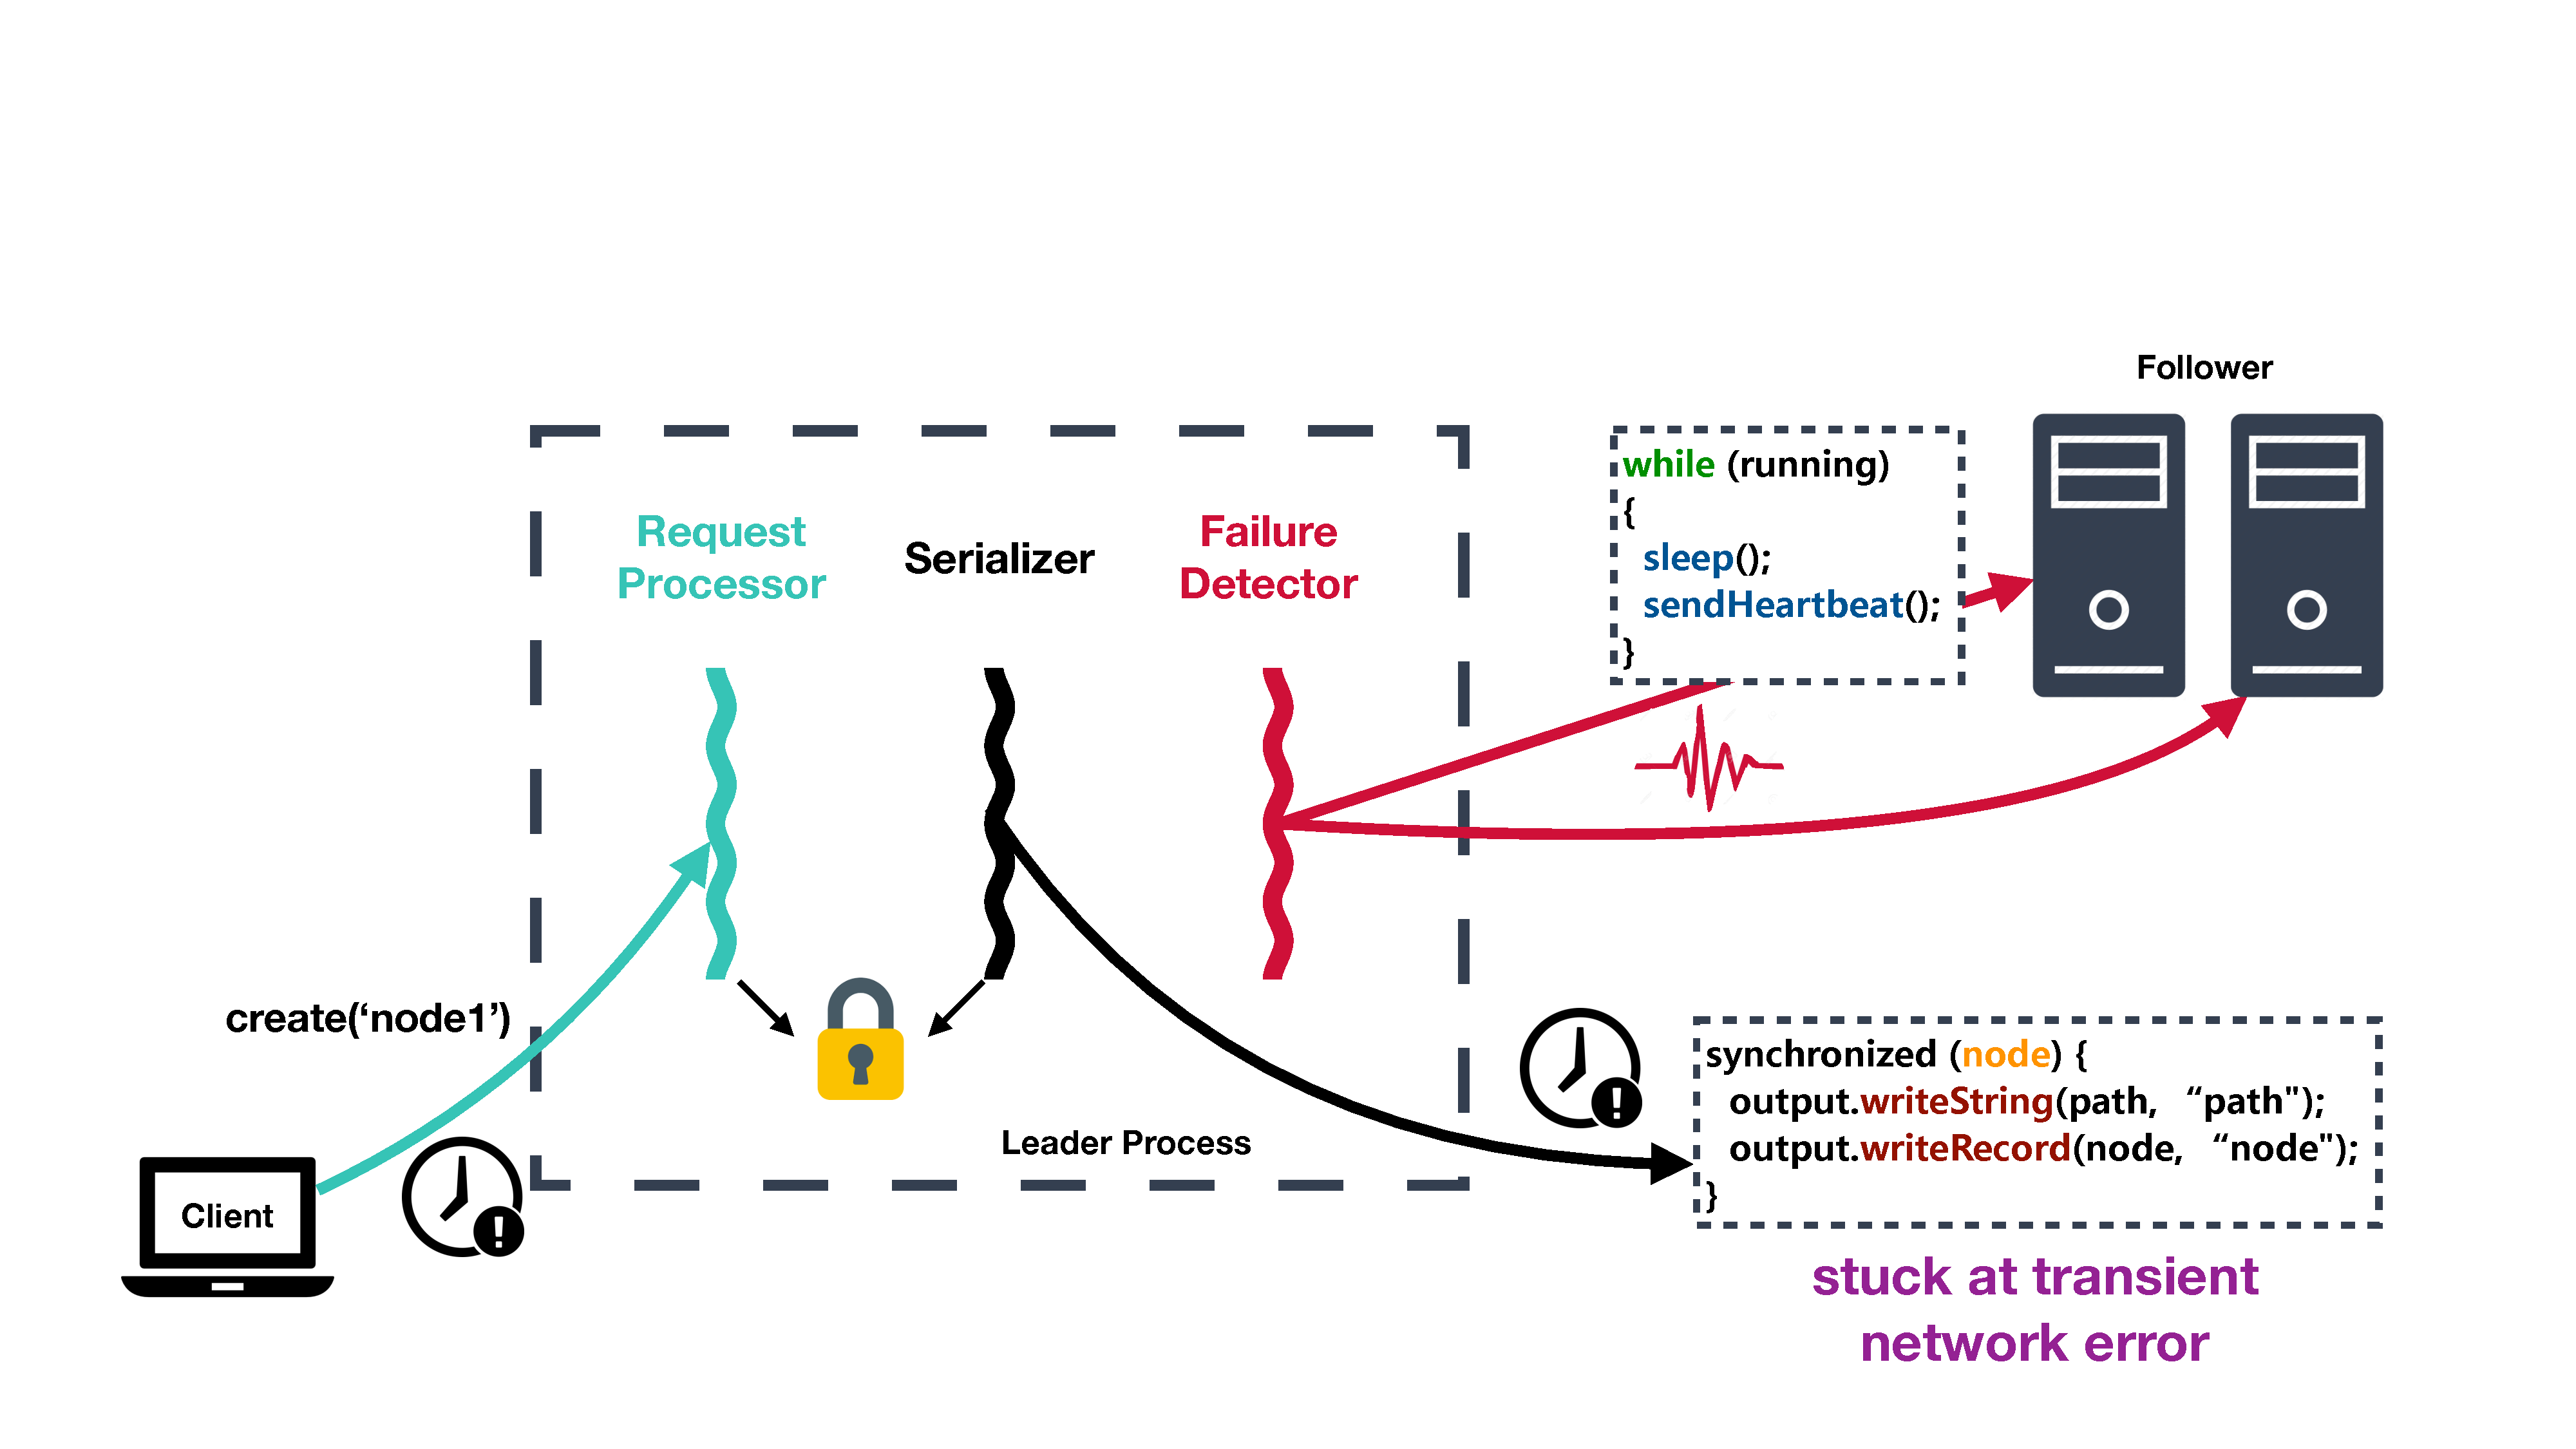
\includegraphics[width=\textwidth]{fig/example1}
    \end{center}
\end{frame}

\begin{frame}
    \frametitle{What is a Partial Failure?}
    \begin{definition}
        A partial failure is, in a process $\pi$ to be when a fault \textbf{does not} crash $\pi$ but causes safety or liveness violation or severe slowness for some functionality $R_f \subsetneq  R$

    \end{definition}
    \textbf{Scope:} In this paper, we will specify the partial failure at the \red{process} granularity instead of \blue{service}.
    \begin{center}
        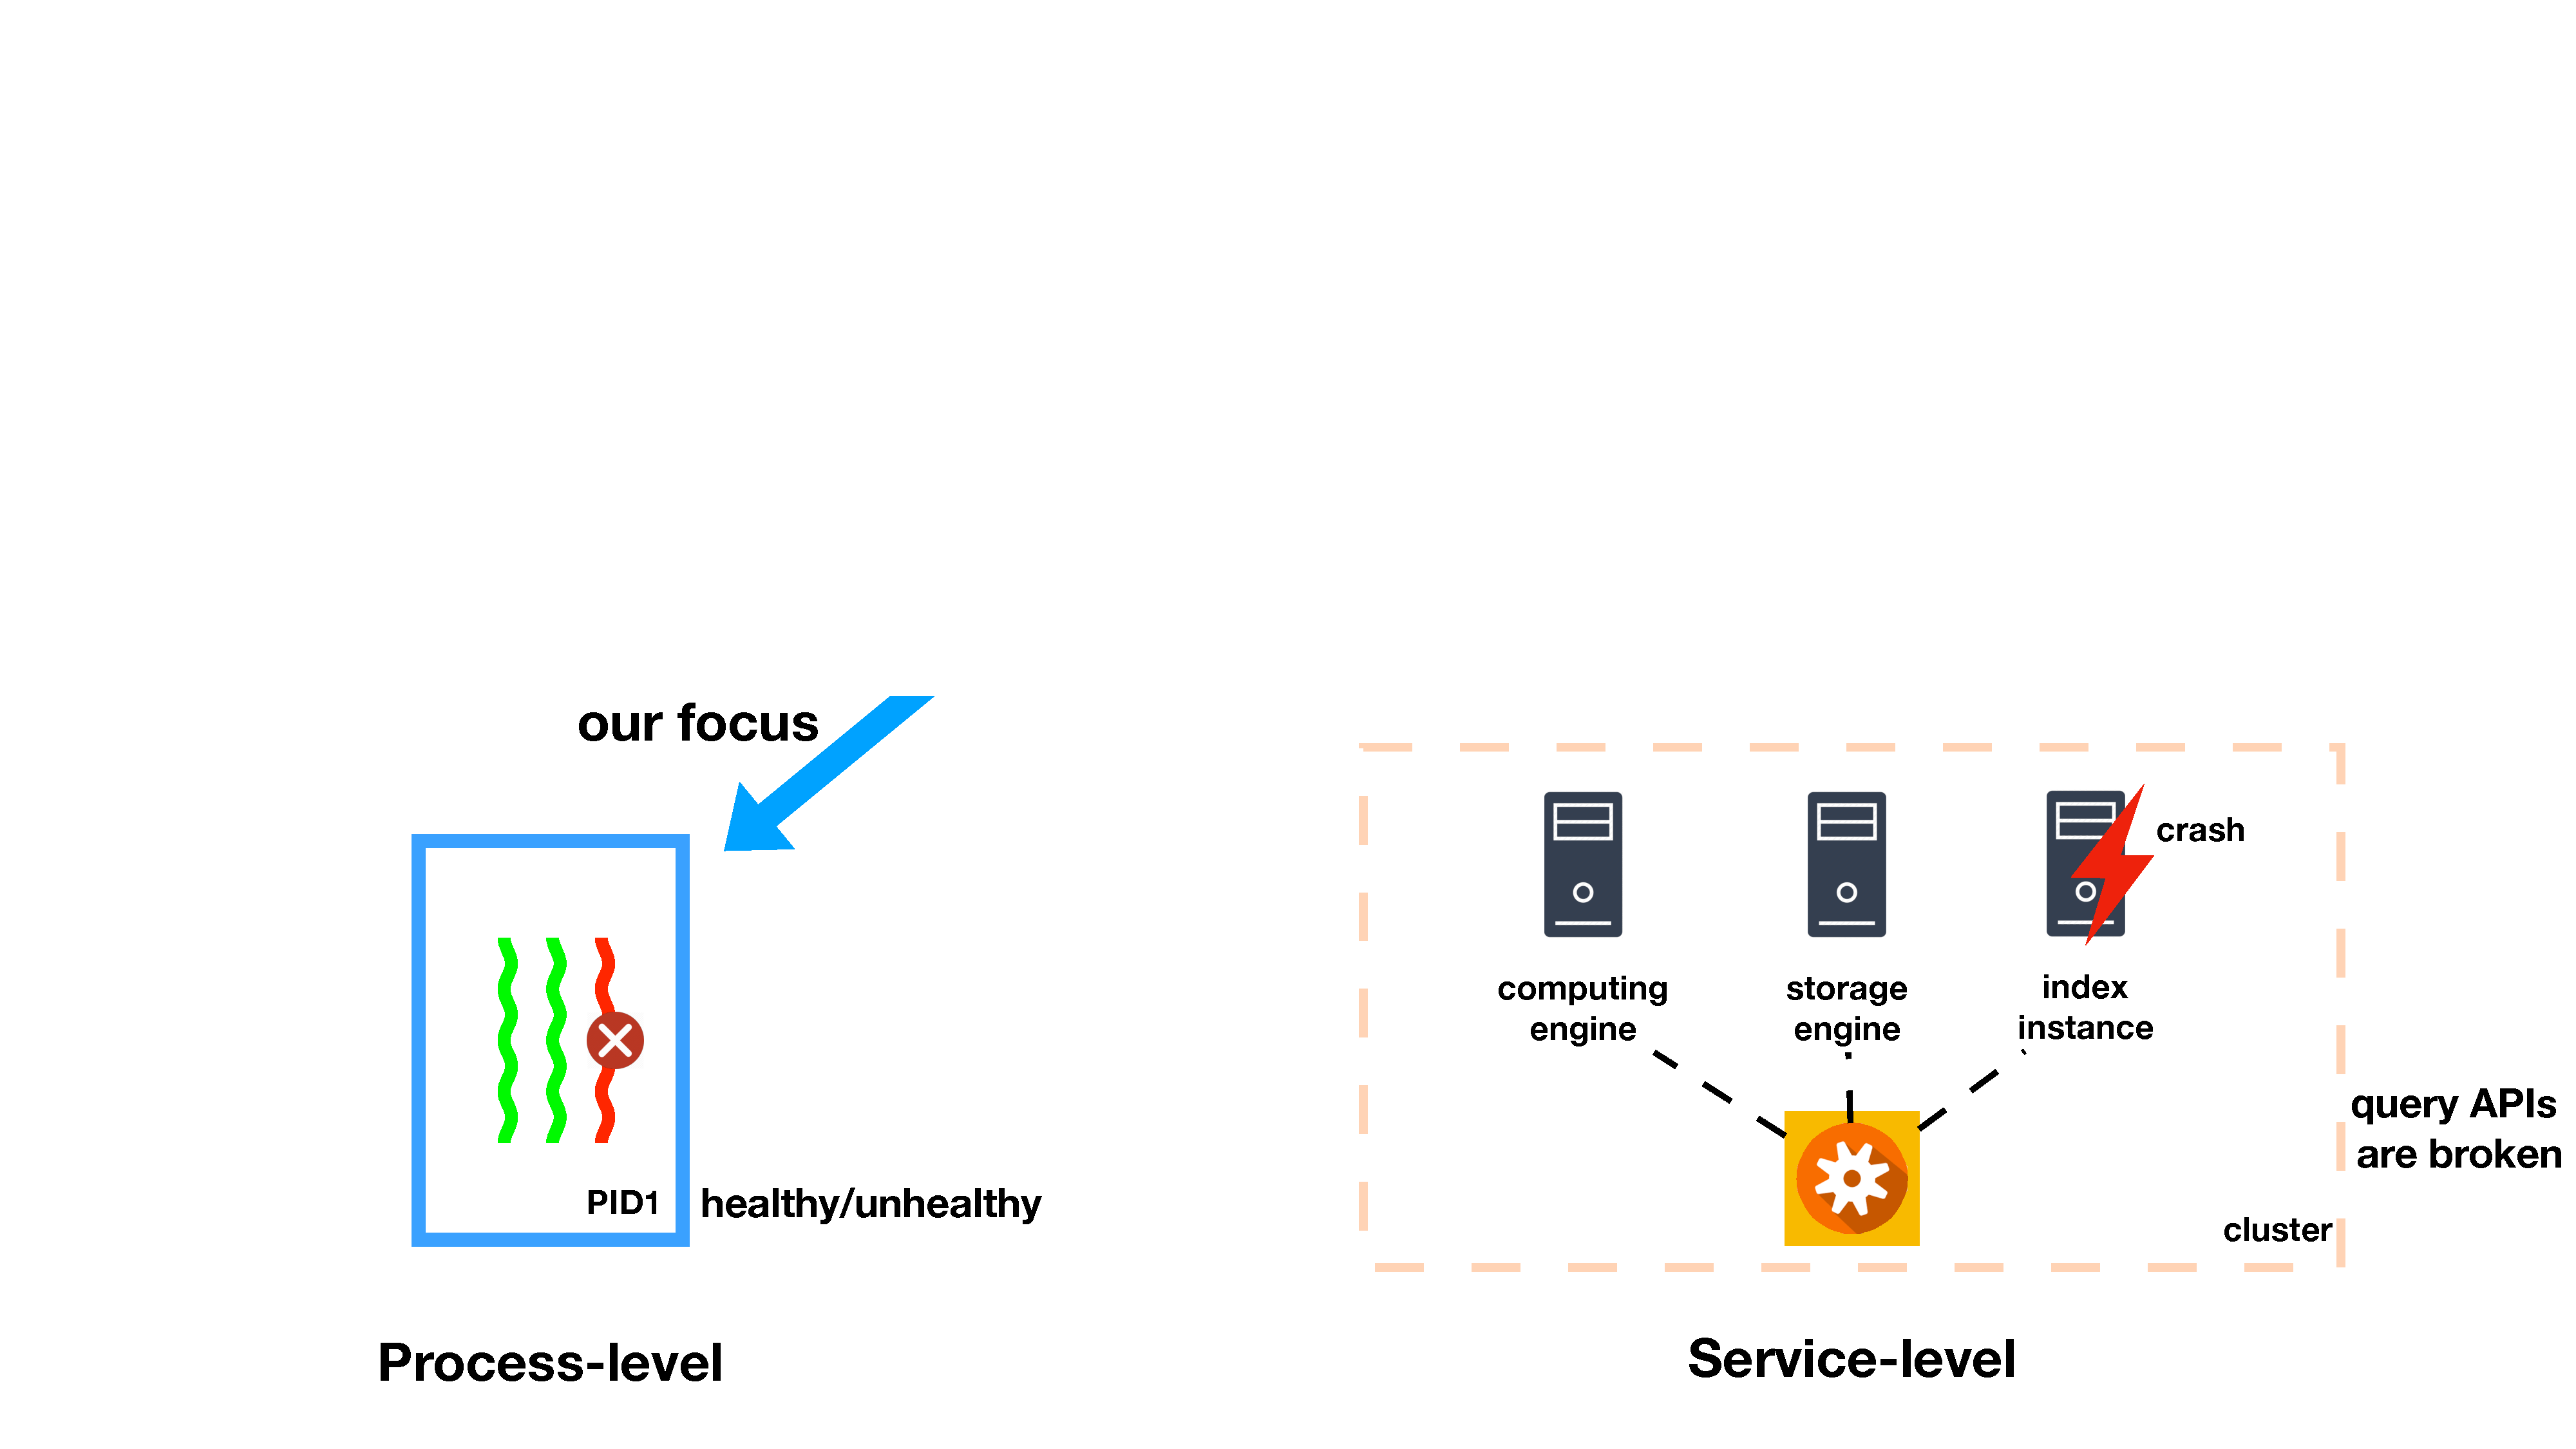
\includegraphics[width=.9\textwidth]{fig/level}
    \end{center}
\end{frame}

\section{Case Study}
\begin{frame}
    \frametitle{Study methodology}
    \begin{block}{\textbf{100 partial failure cases from five large, widely-used software systems}}
        \begin{itemize}
            \item Crawl all bug tickets tagged with critical priorities in the official
                  bug trackers
            \item Filter tickets from testing and randomly
                  sample the remaining failures tickets.
        \end{itemize}
    \end{block}

    Interestingly, \red{54\%} of them occur in the most recent \red{three} years’ software
    releases \textit{(average lifespan of all systems is \red{9} years)}
    \begin{center}
        \begin{tabular}{c|c|c|c|c}
            \toprule
            Software  & Language & Cases & Versions           & Date Range            \\
            \midrule
            ZooKeeper & Java     & 20    & 17 (3.2.1–3.5.3)   & 12/01/2009–08/28/2018 \\
            Cassandra & Java     & 20    & 19 (0.7.4–3.0.13)  & 04/22/2011–08/31/2017 \\
            HDFS      & Java     & 20    & 14 (0.20.1–3.1.0)  & 10/29/2009–08/06/2018 \\
            Apache    & C        & 20    & 16 (2.0.40–2.4.29) & 08/02/2002–03/20/2018 \\
            Mesos     & C++      & 20    & 11 (0.11.0–1.7.0)  & 04/08/2013–12/28/2018 \\
            \bottomrule
        \end{tabular}
    \end{center}
\end{frame}

\subsection{Findings}

\begin{frame}
    \frametitle{Finding 1: Root Causes are \red{Diverse}}
    \framesubtitle{Root cause distribution}
    \begin{block}{\textbf{\red{No} single uniformed or dominating root cause}\footnote{UE: uncaught error; IB: indefinite blocking; EH: buggy error handling;
                DD: deadlock; PB: performance bug; LE: logic error; IL: infinite loop; RL: resource leak.}}
        Top three (total \red{48\%}) root cause types are \blue{uncaught errors},\blue{indefinite blocking}, and \blue{buggy error handling}
    \end{block}

    \begin{center}
        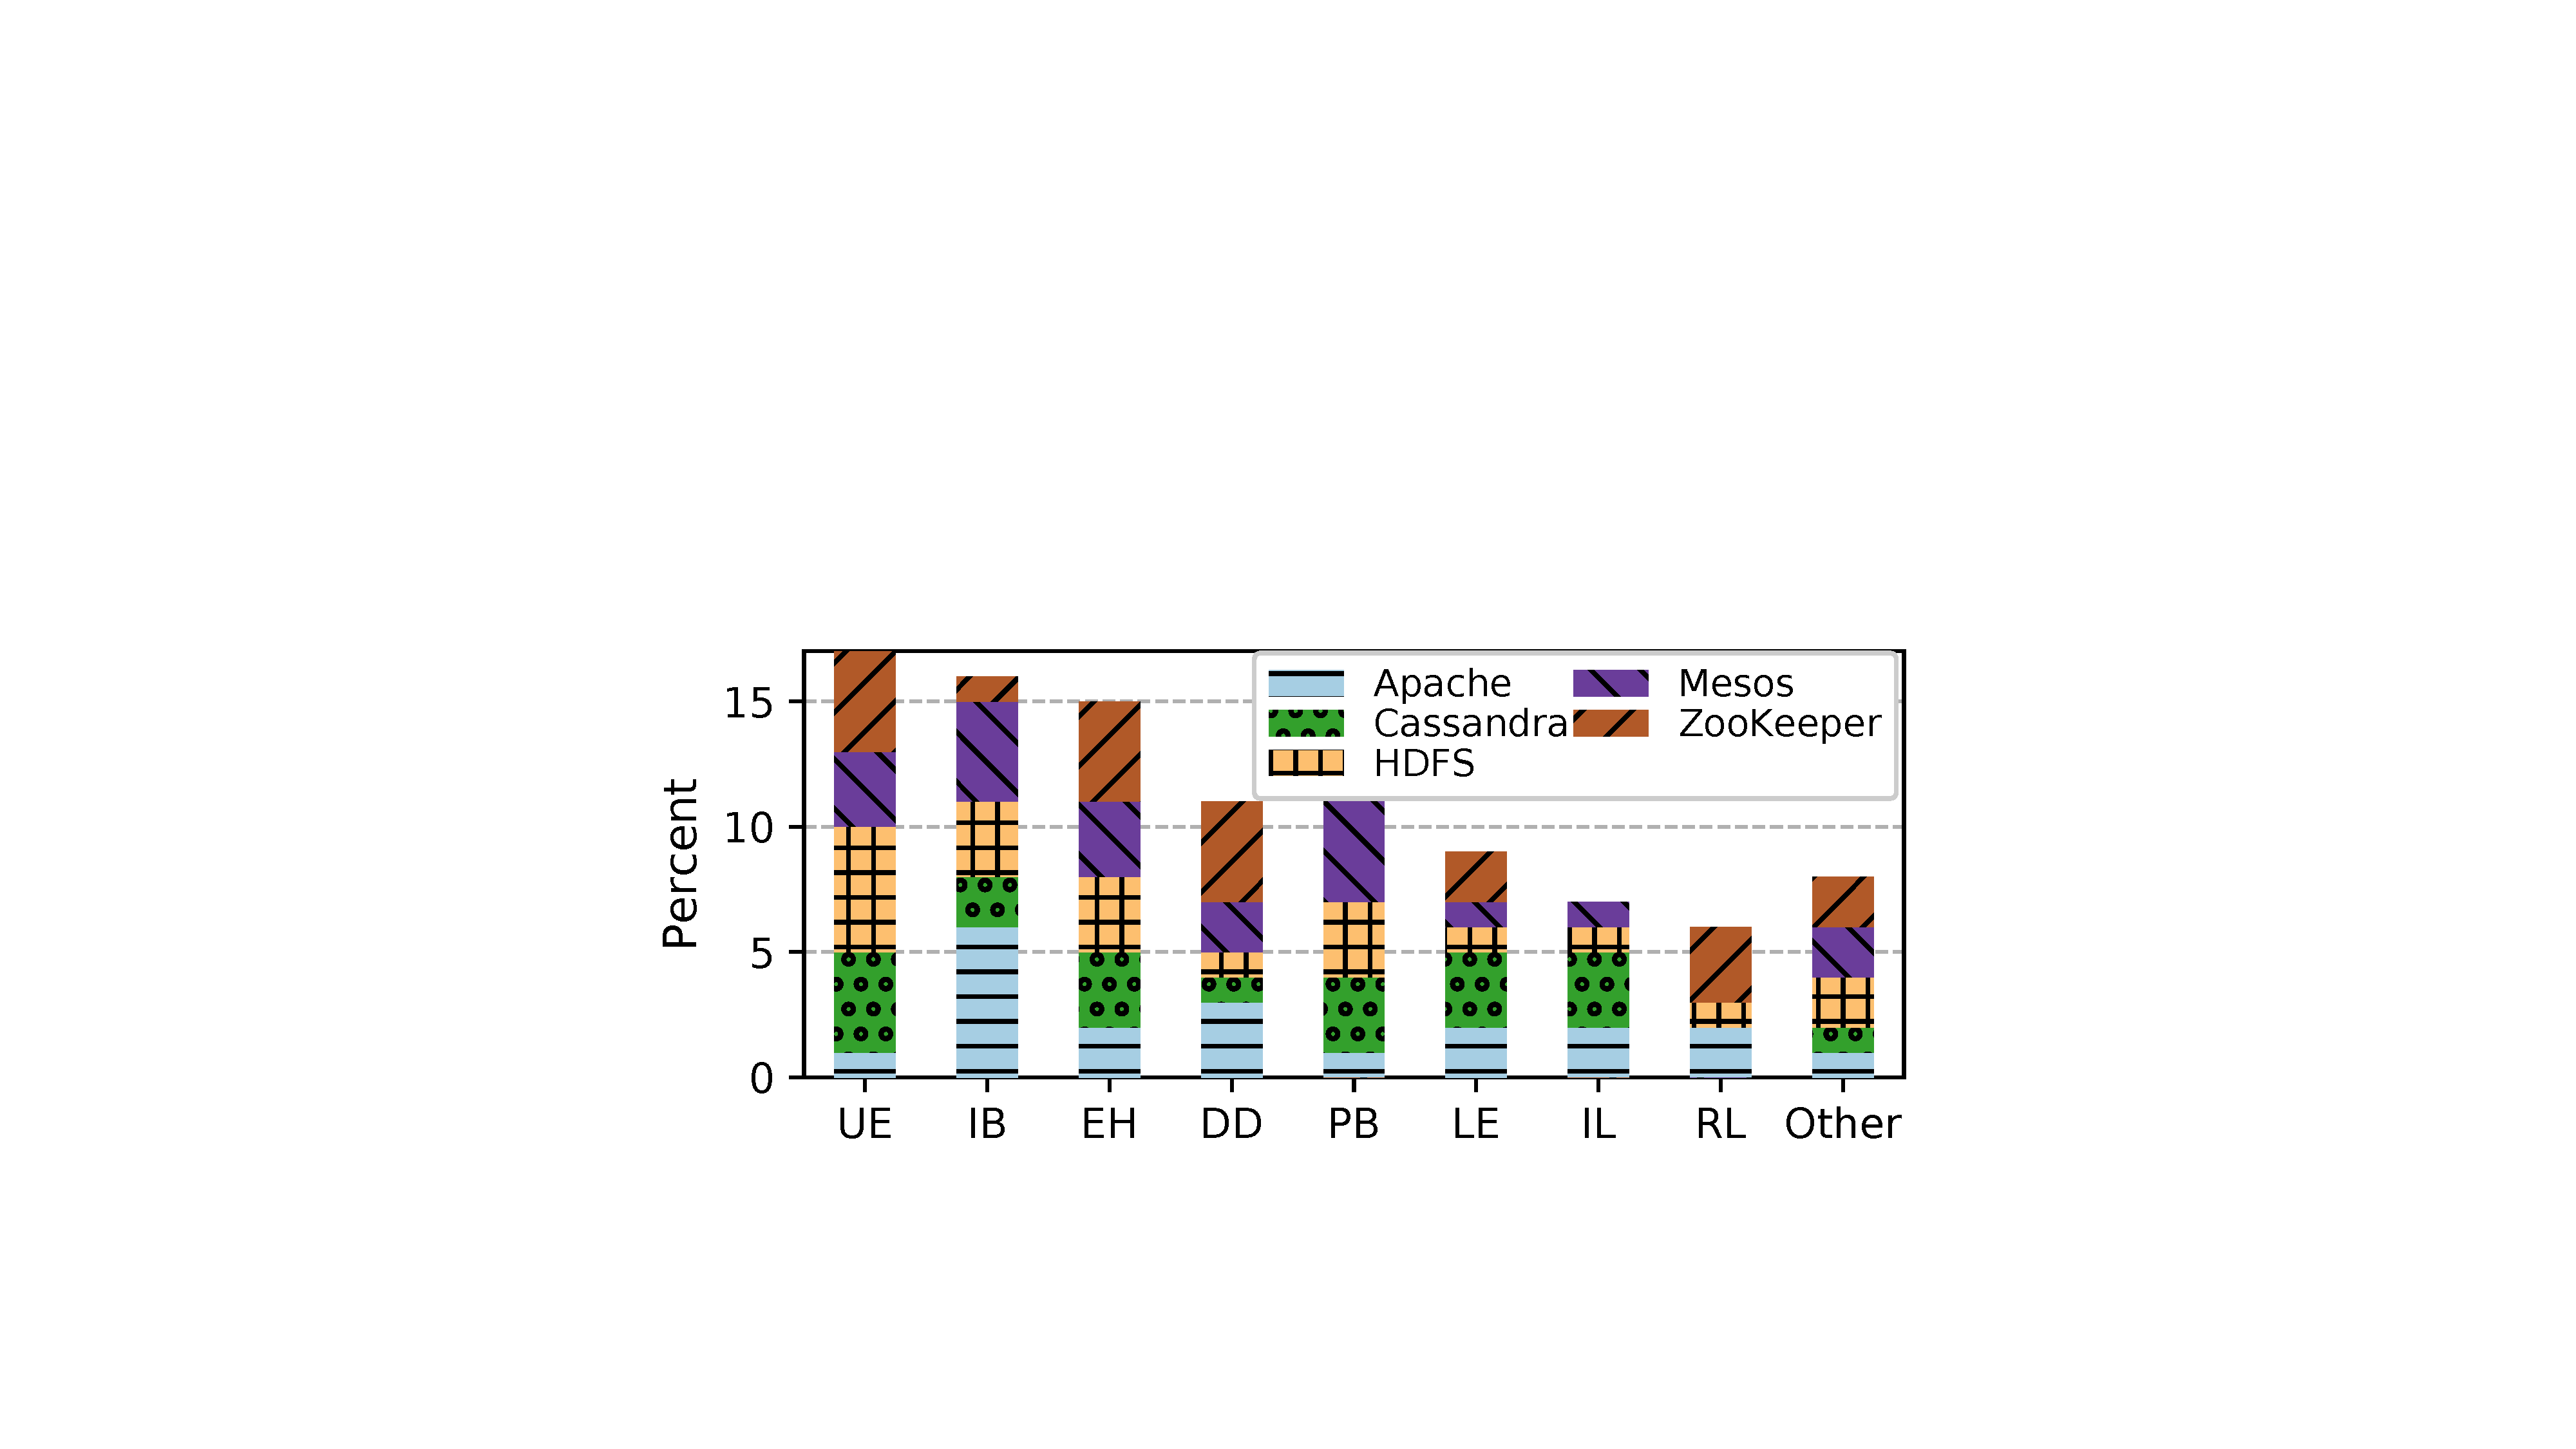
\includegraphics[width=.75\textwidth]{fig/root-cause}
    \end{center}
\end{frame}

\begin{frame}
    \frametitle{Finding 2: Nearly Half Cases Cause \red{Stuck} Issues}
    \framesubtitle{Consequence}
    Nearly half (\red{48\%}) of the partial failures cause some functionality to be \textit{\red{stuck}}.
    \begin{center}
        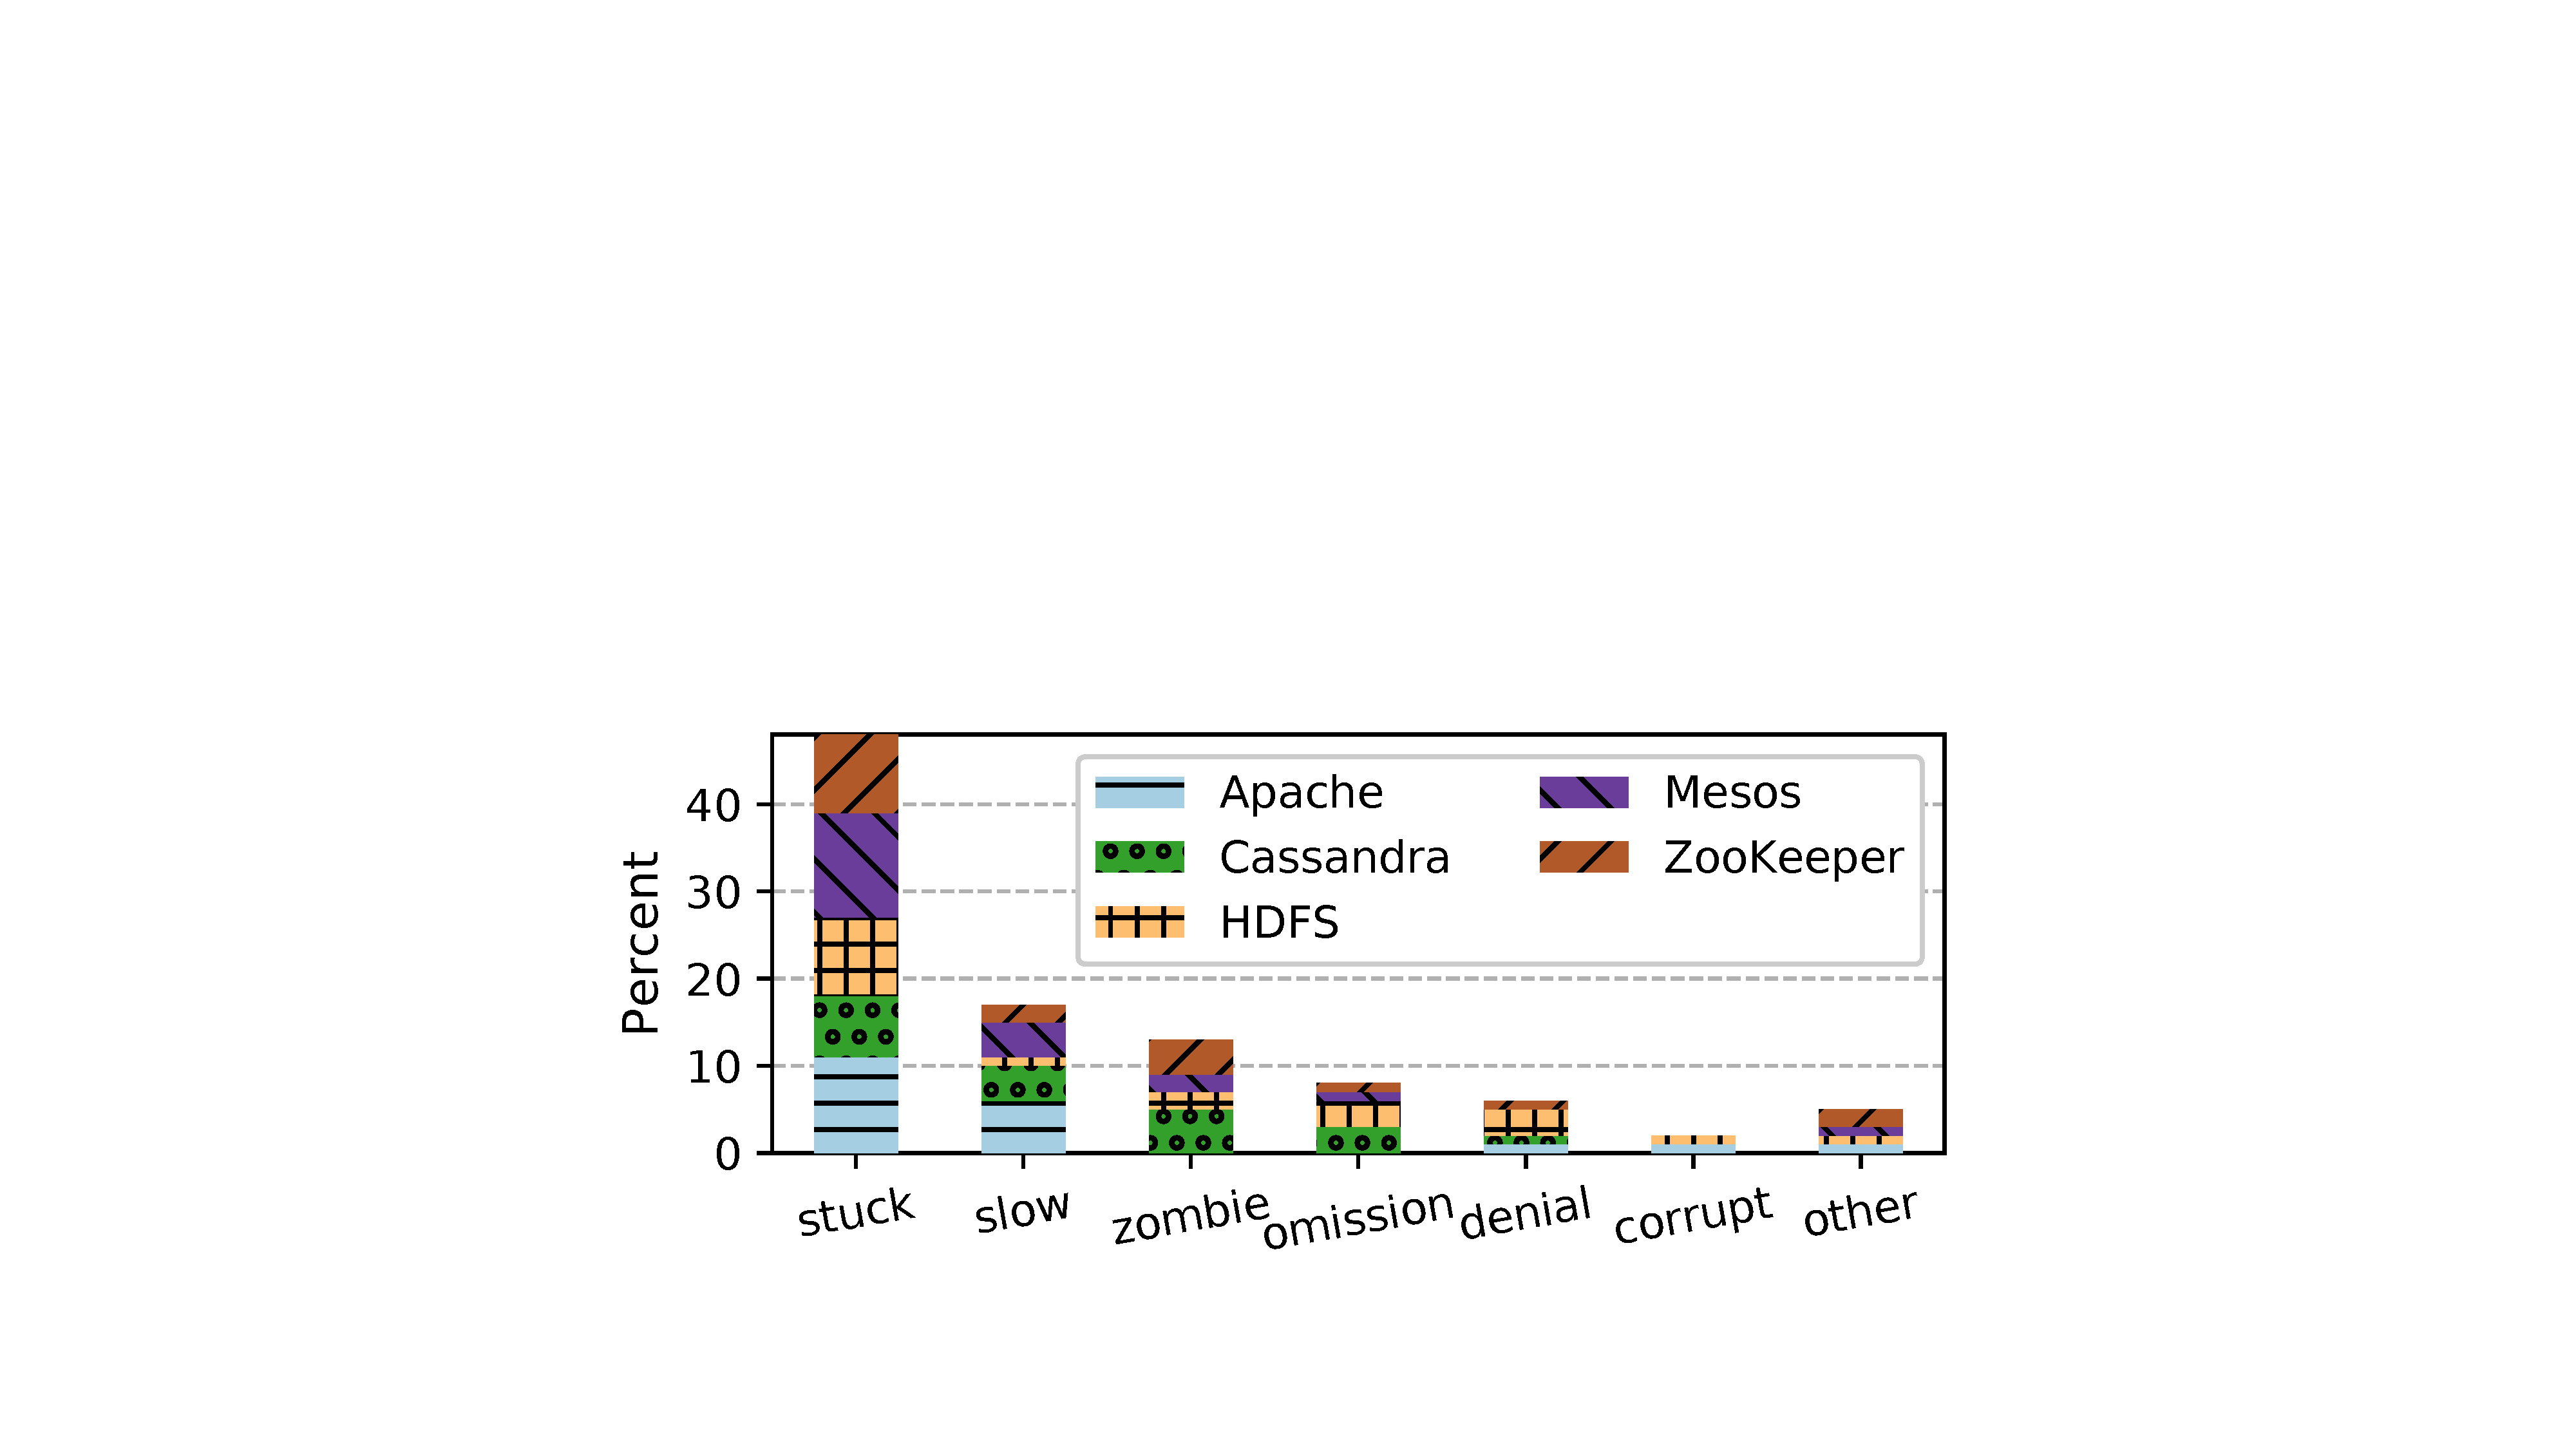
\includegraphics[width=.75\textwidth]{fig/consequence}
    \end{center}

    \red{17\%} of the partial failures cause certain operations to take a long time to complete. (i.e. \blue{\textit{slow}})
\end{frame}

\begin{frame}
    \frametitle{Other Findings: Partial Failures are Hard to Detect}
    \begin{block}{\textbf{\red{15\%} of the partial failures are silent}}
        Including data loss,corruption, inconsistency, and wrong results
    \end{block}

    \begin{block}{\textbf{\red{Most} cases are triggered by unique production workload or environment}}
        \red{71\%} of the partial failures are triggered by some \textbf{specific
            environment condition}, or \textbf{special input} in the \textbf{production}.
    \end{block}

    \begin{block}{\textbf{Debugging time is \red{long}}}
        The median diagnosis time is 6 days and 5 hours
    \end{block}

    \begin{block}{\textbf{The \red{majority (68\%)} of the failures are \red{“sticky”}}}
        The process will not recover from the faults by itself. The faulty process needs to be restarted or repaired to function again.
    \end{block}
\end{frame}

\section{Motivation}

\begin{frame}
    \frametitle{Motivation}
    What if we simply apply static or dynamic analysis?
    \framesubtitle{So how to detect and localize a partial failure in a big software?}
    \begin{columns}
        \begin{column}{.5\textwidth}


            \begin{block}{Static Analysis?}
                \begin{itemize}
                    \item no unique production env/workload
                    \item unable to detect run-time problem
                \end{itemize}
            \end{block}



        \end{column}

        \begin{column}{.48\textwidth}
            \begin{block}{Dynamic Analysis?}
                \begin{itemize}
                    \item existing detectors are too shallow
                    \item unable to  localize failures
                \end{itemize}
            \end{block}
        \end{column}
    \end{columns}

    \vspace{1em}

    Ask developers to manually add defensive checks?

    \begin{block}{Manual vs generated checkers}
        \textbf{Systematically} generated checkers to ease developers’ burden
        \begin{itemize}
            \item challenge: difficult to automate for all cases
            \item opportunity: most of partial failures do not rely on deep semantic understanding
                  to detect, such checkers can potentially be automatically constructed
        \end{itemize}
    \end{block}
\end{frame}

\section{Proposed Design}

\subsection{Ideas}

\begin{frame}
    \frametitle{Intersection Principle}

    Construct
    customized checkers that \textbf{intersect} with the execution of a monitored process:

    \begin{center}
        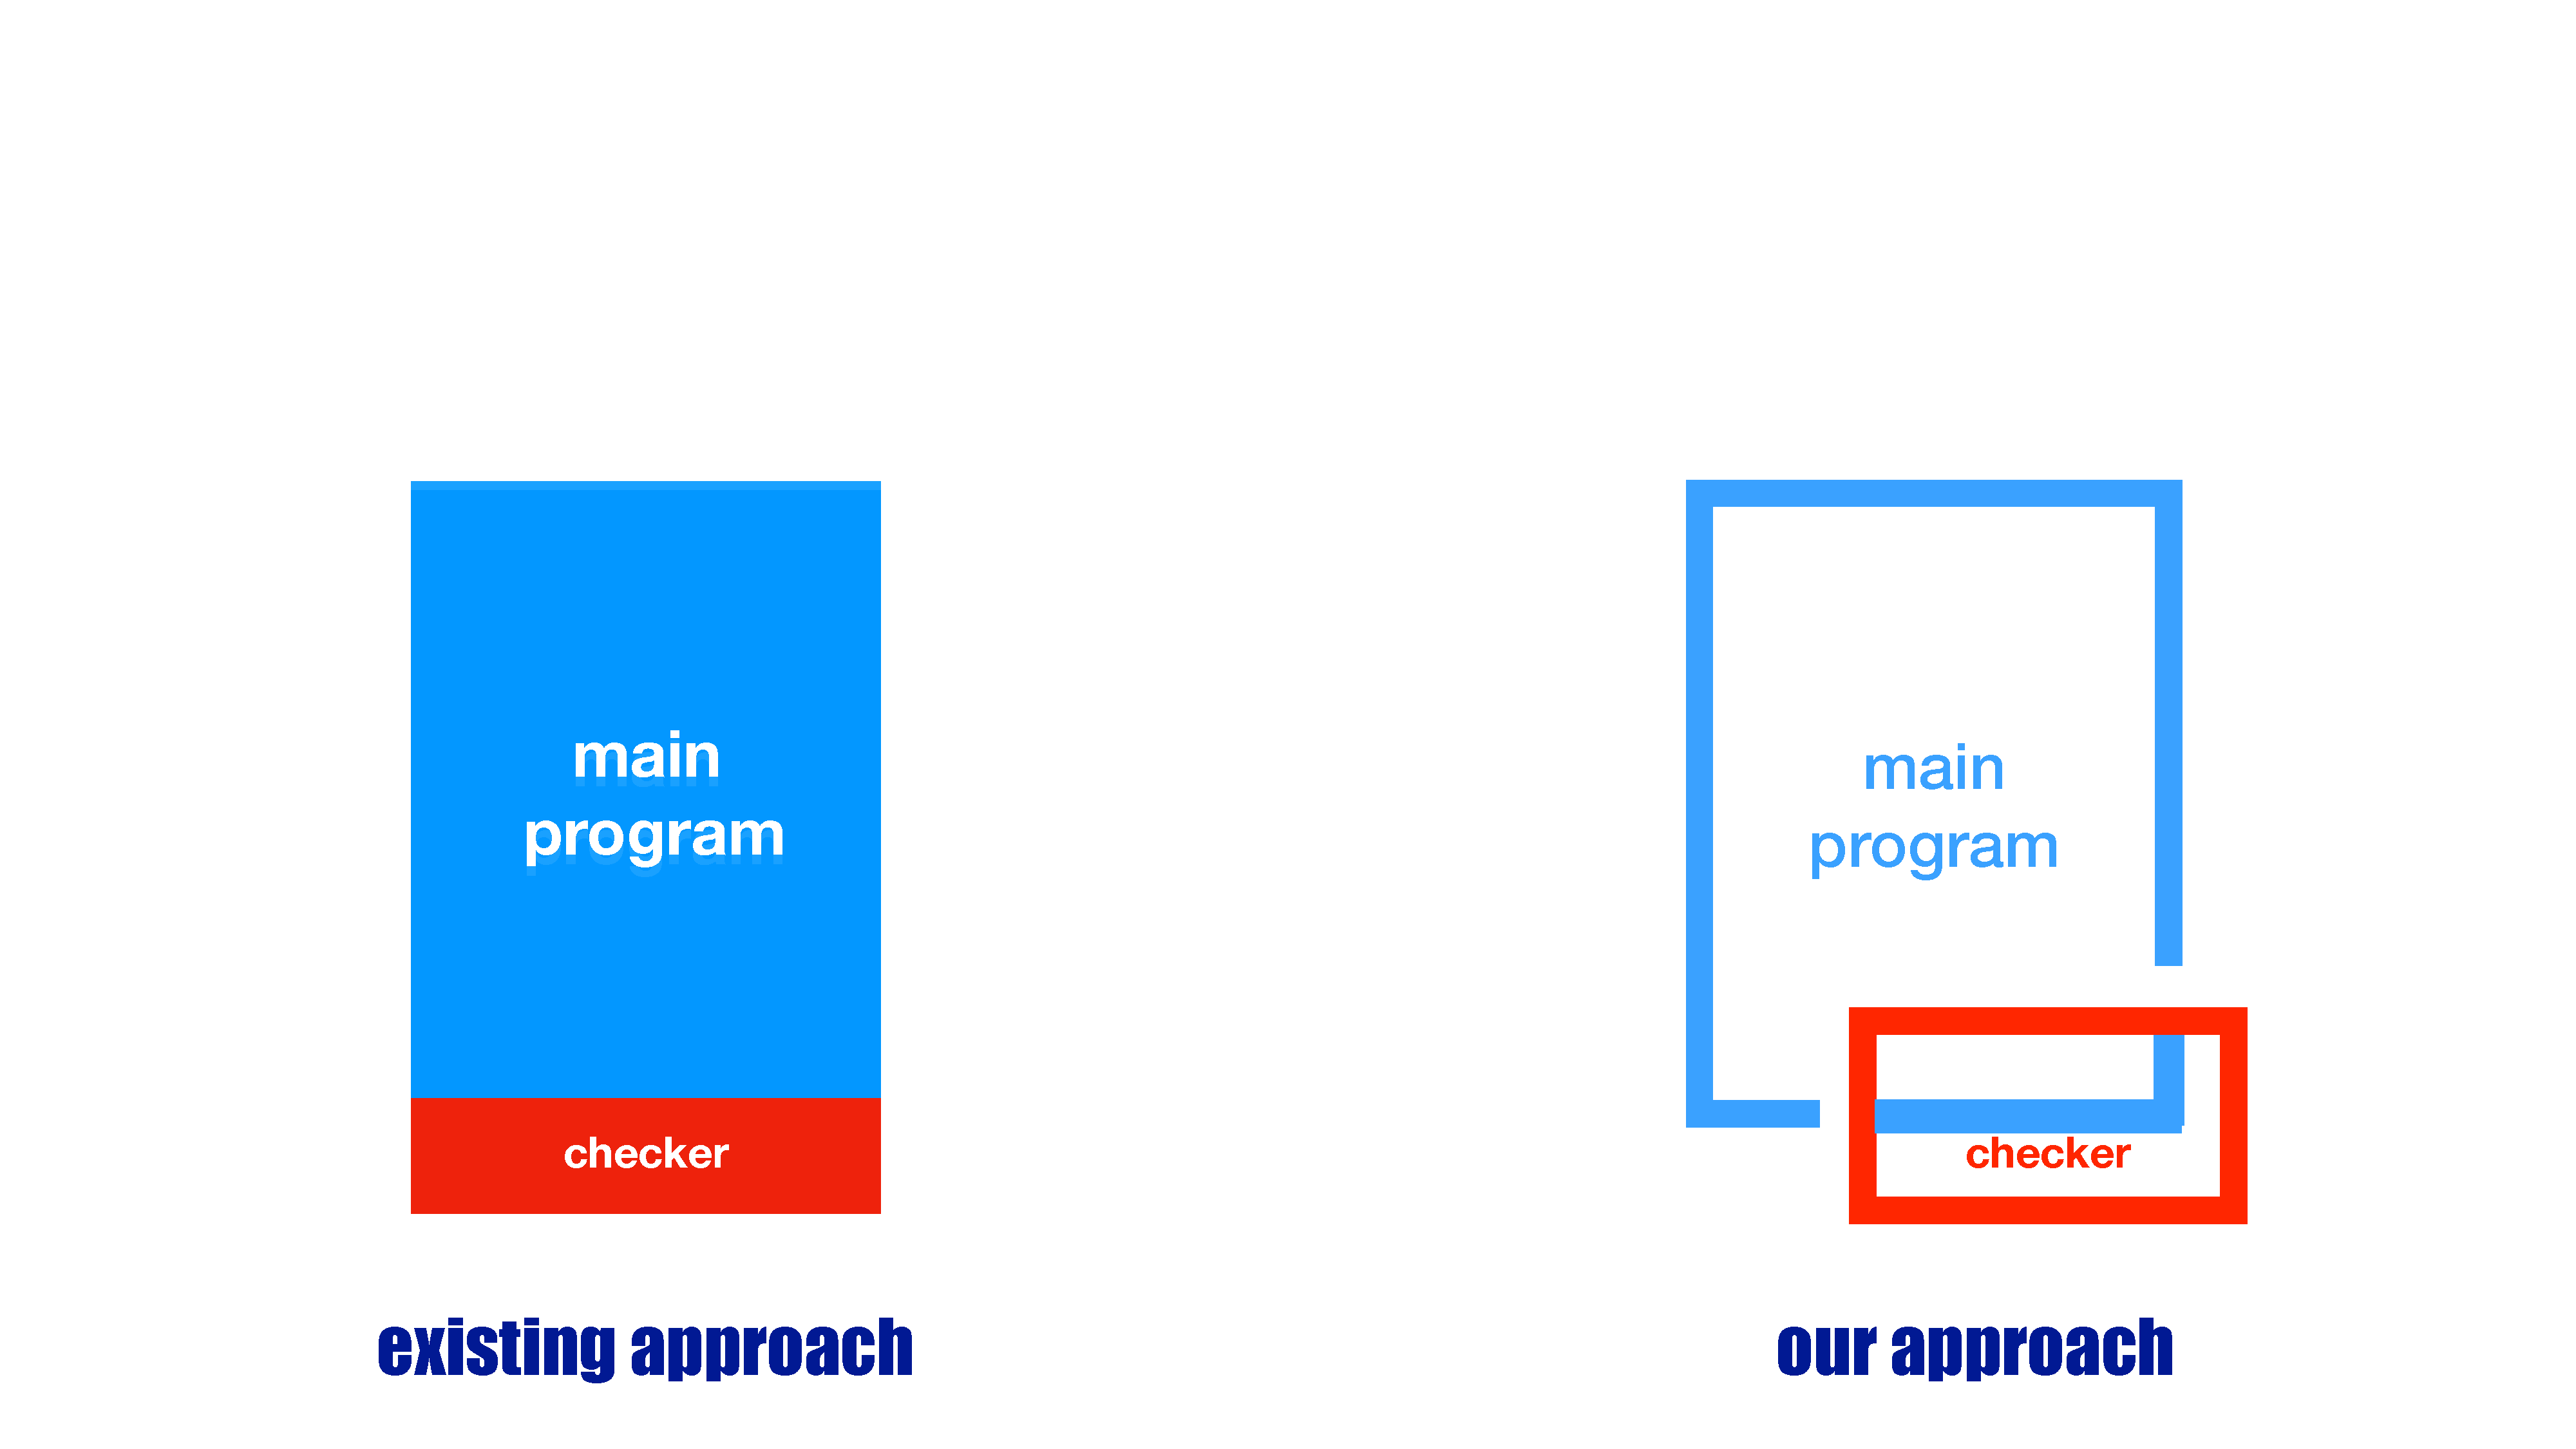
\includegraphics[width=.85\textwidth]{fig/intersect.pdf}
    \end{center}
\end{frame}

\begin{frame}
    \frametitle{Intrinsic watchdog: Runtime}
    % \framesubtitle{Follows Intersection Principle}
    An intrinsic watchdog is a dedicated monitoring extension for a process

    \begin{center}
        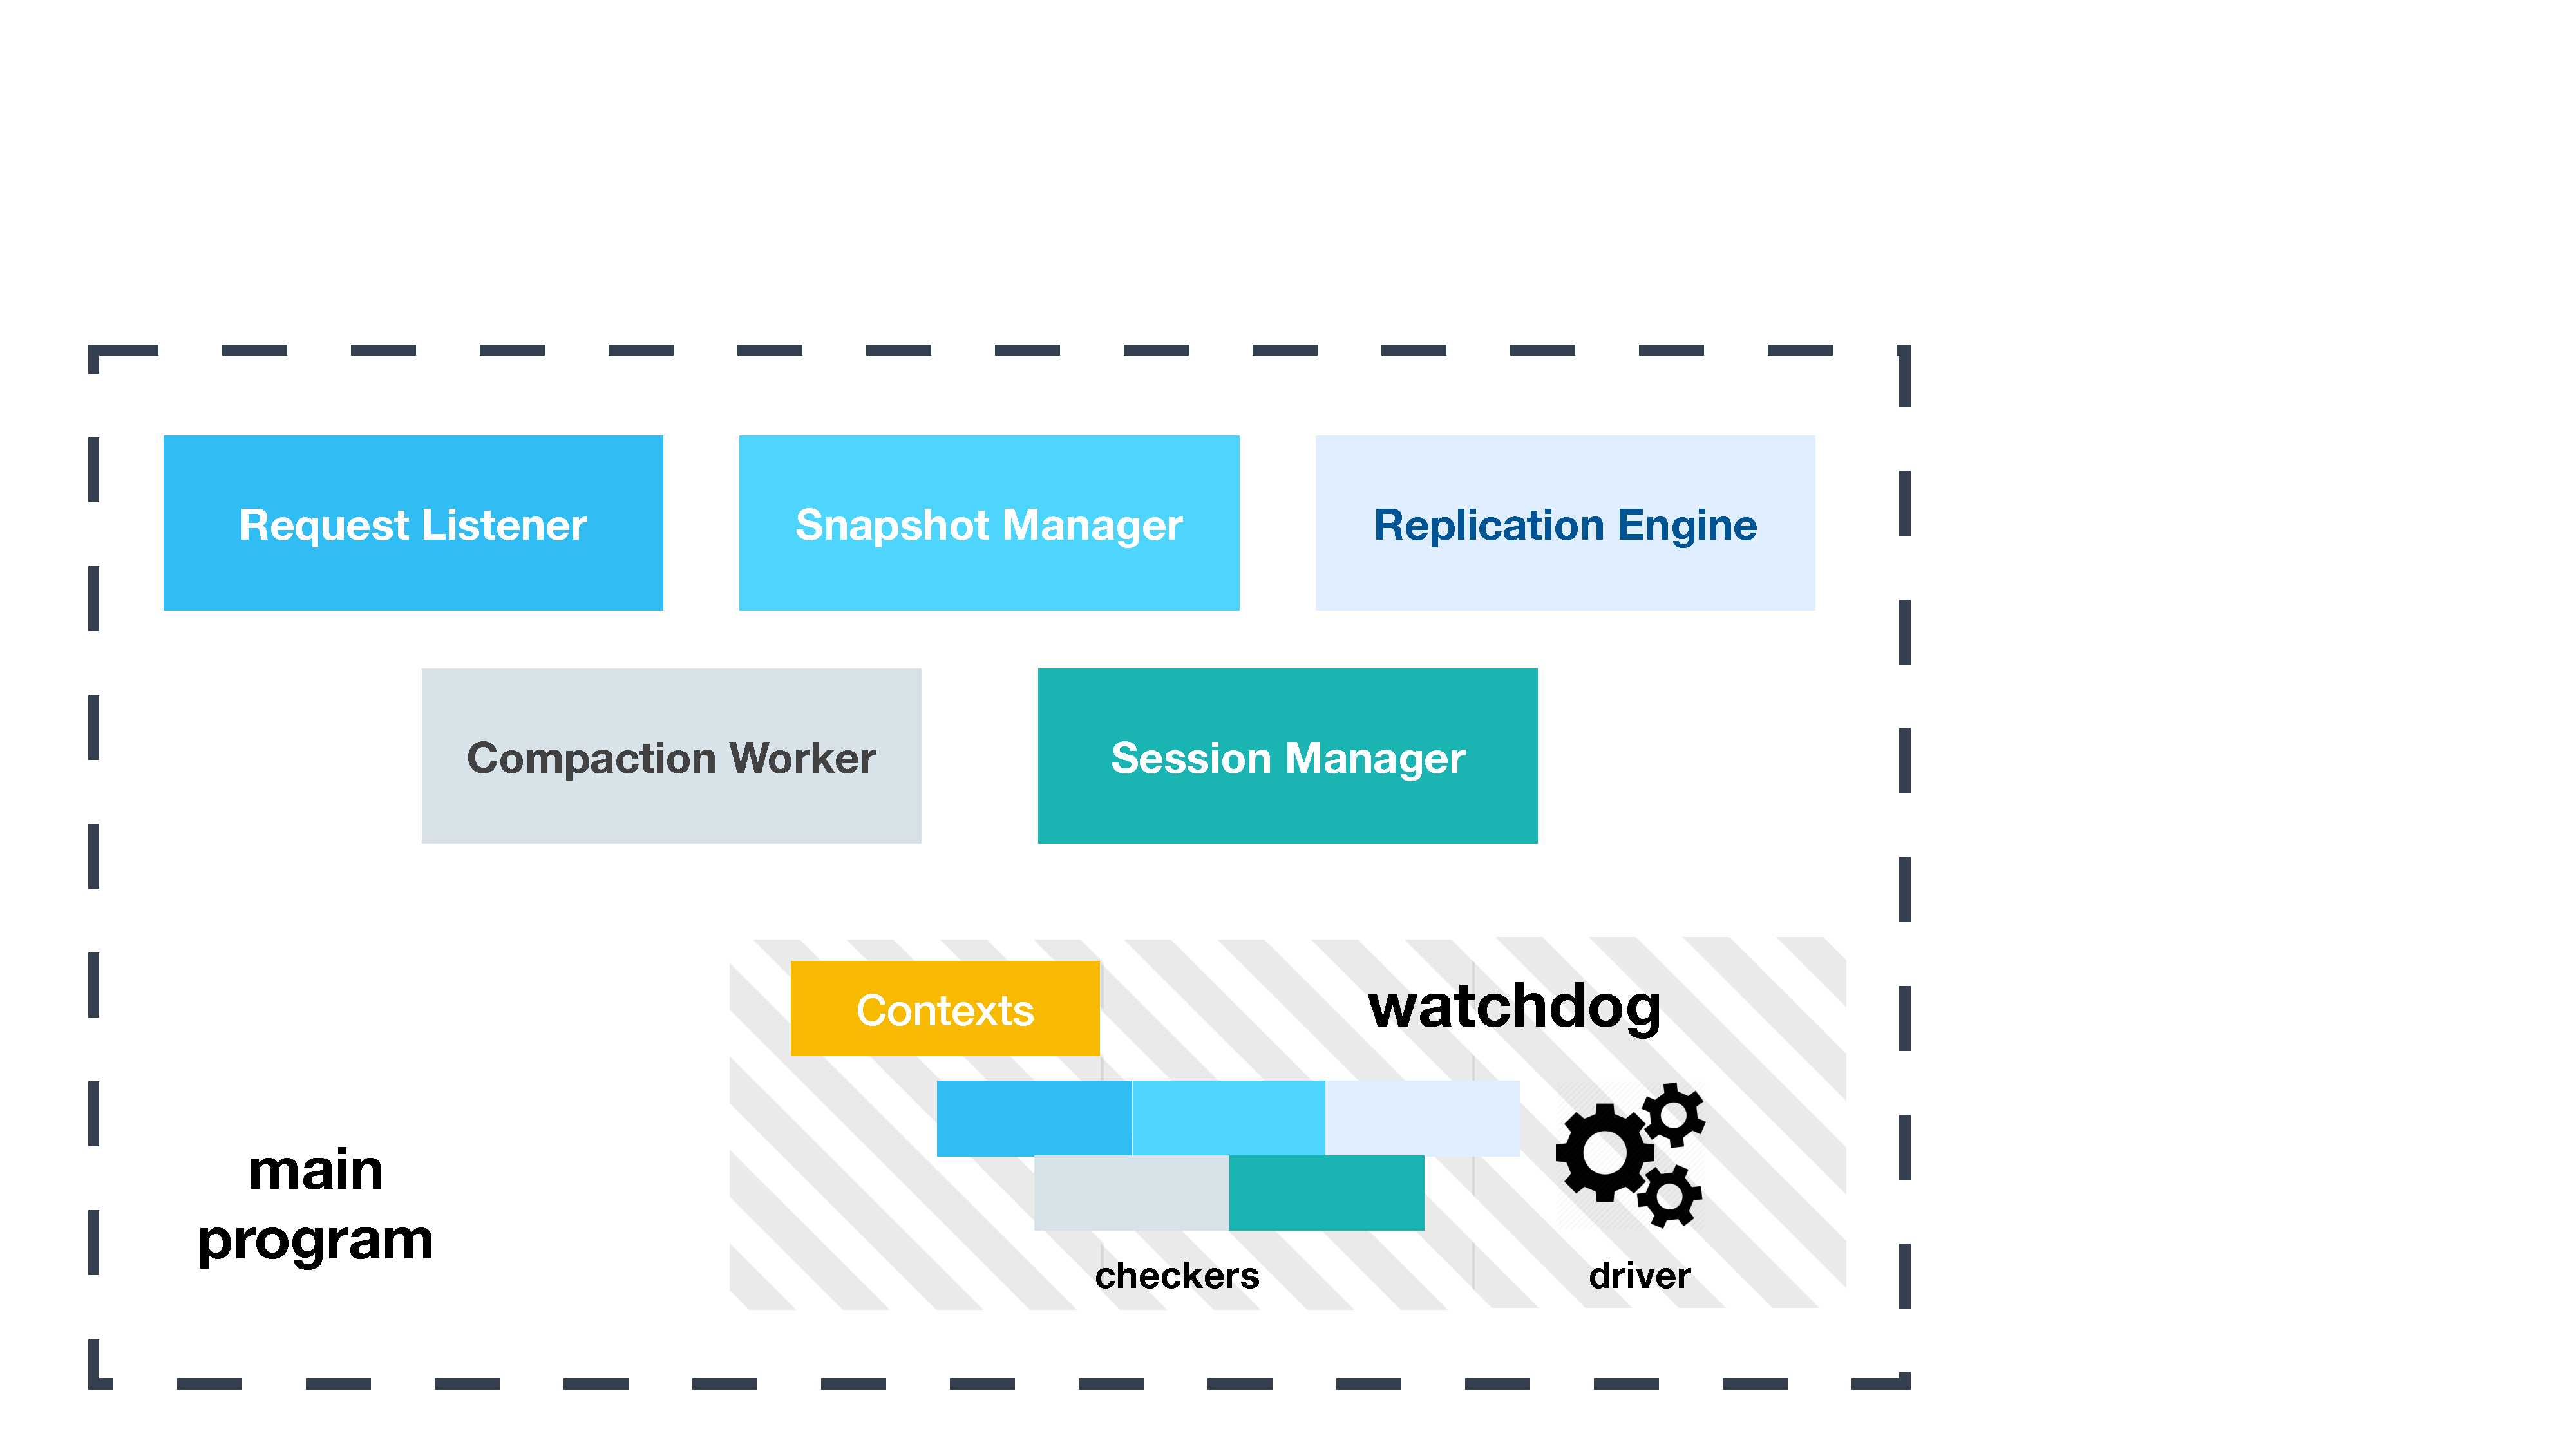
\includegraphics[width=.75\textwidth]{fig/watchdog.pdf}
    \end{center}
\end{frame}

\begin{frame}
    \frametitle{Intrinsic watchdog: How it works?}

    \begin{center}
        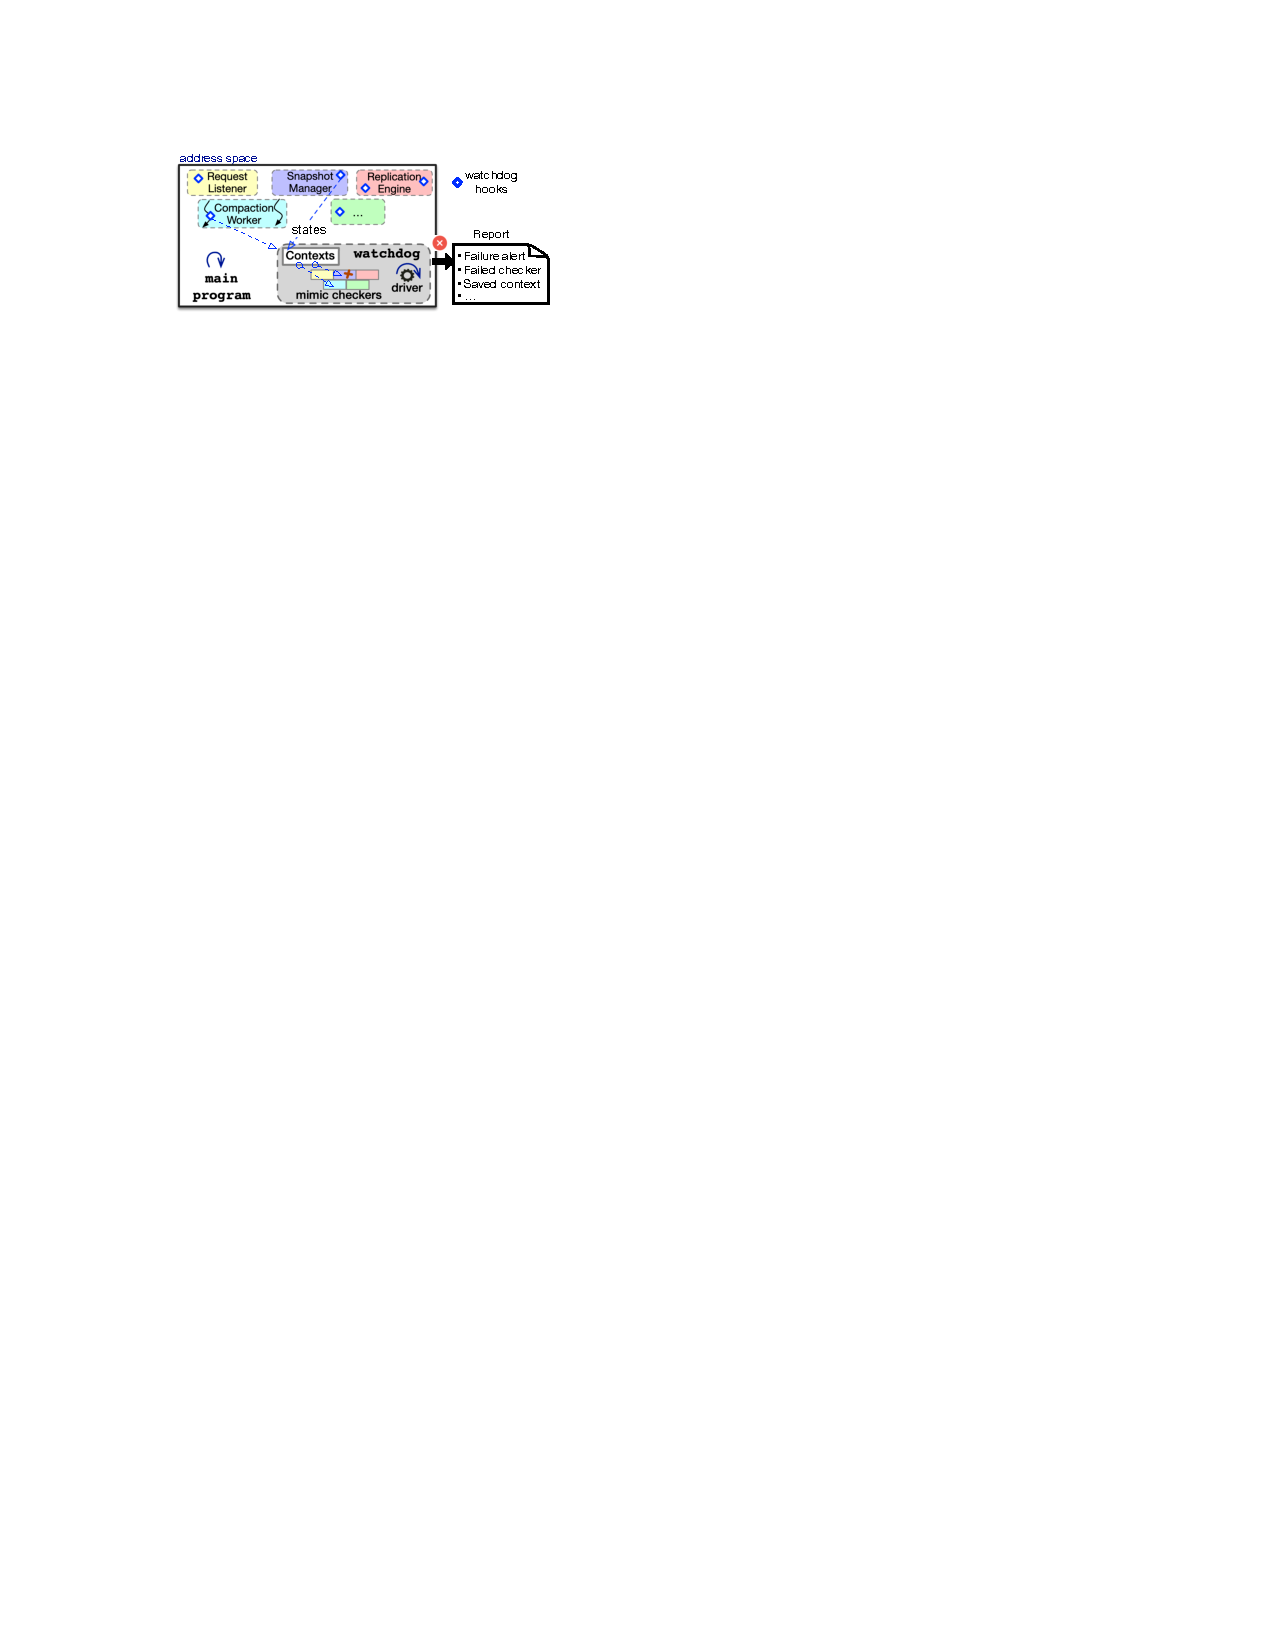
\includegraphics[width=.9\textwidth]{fig/exmaple}
    \end{center}

\end{frame}

\begin{frame}{Characteristic I: Customized}
    \begin{itemize}
        \item Regularly executes a set of checkers tailored to different modules
        \item Selects some representative operations from each
        module
    \end{itemize}

    \begin{center}
        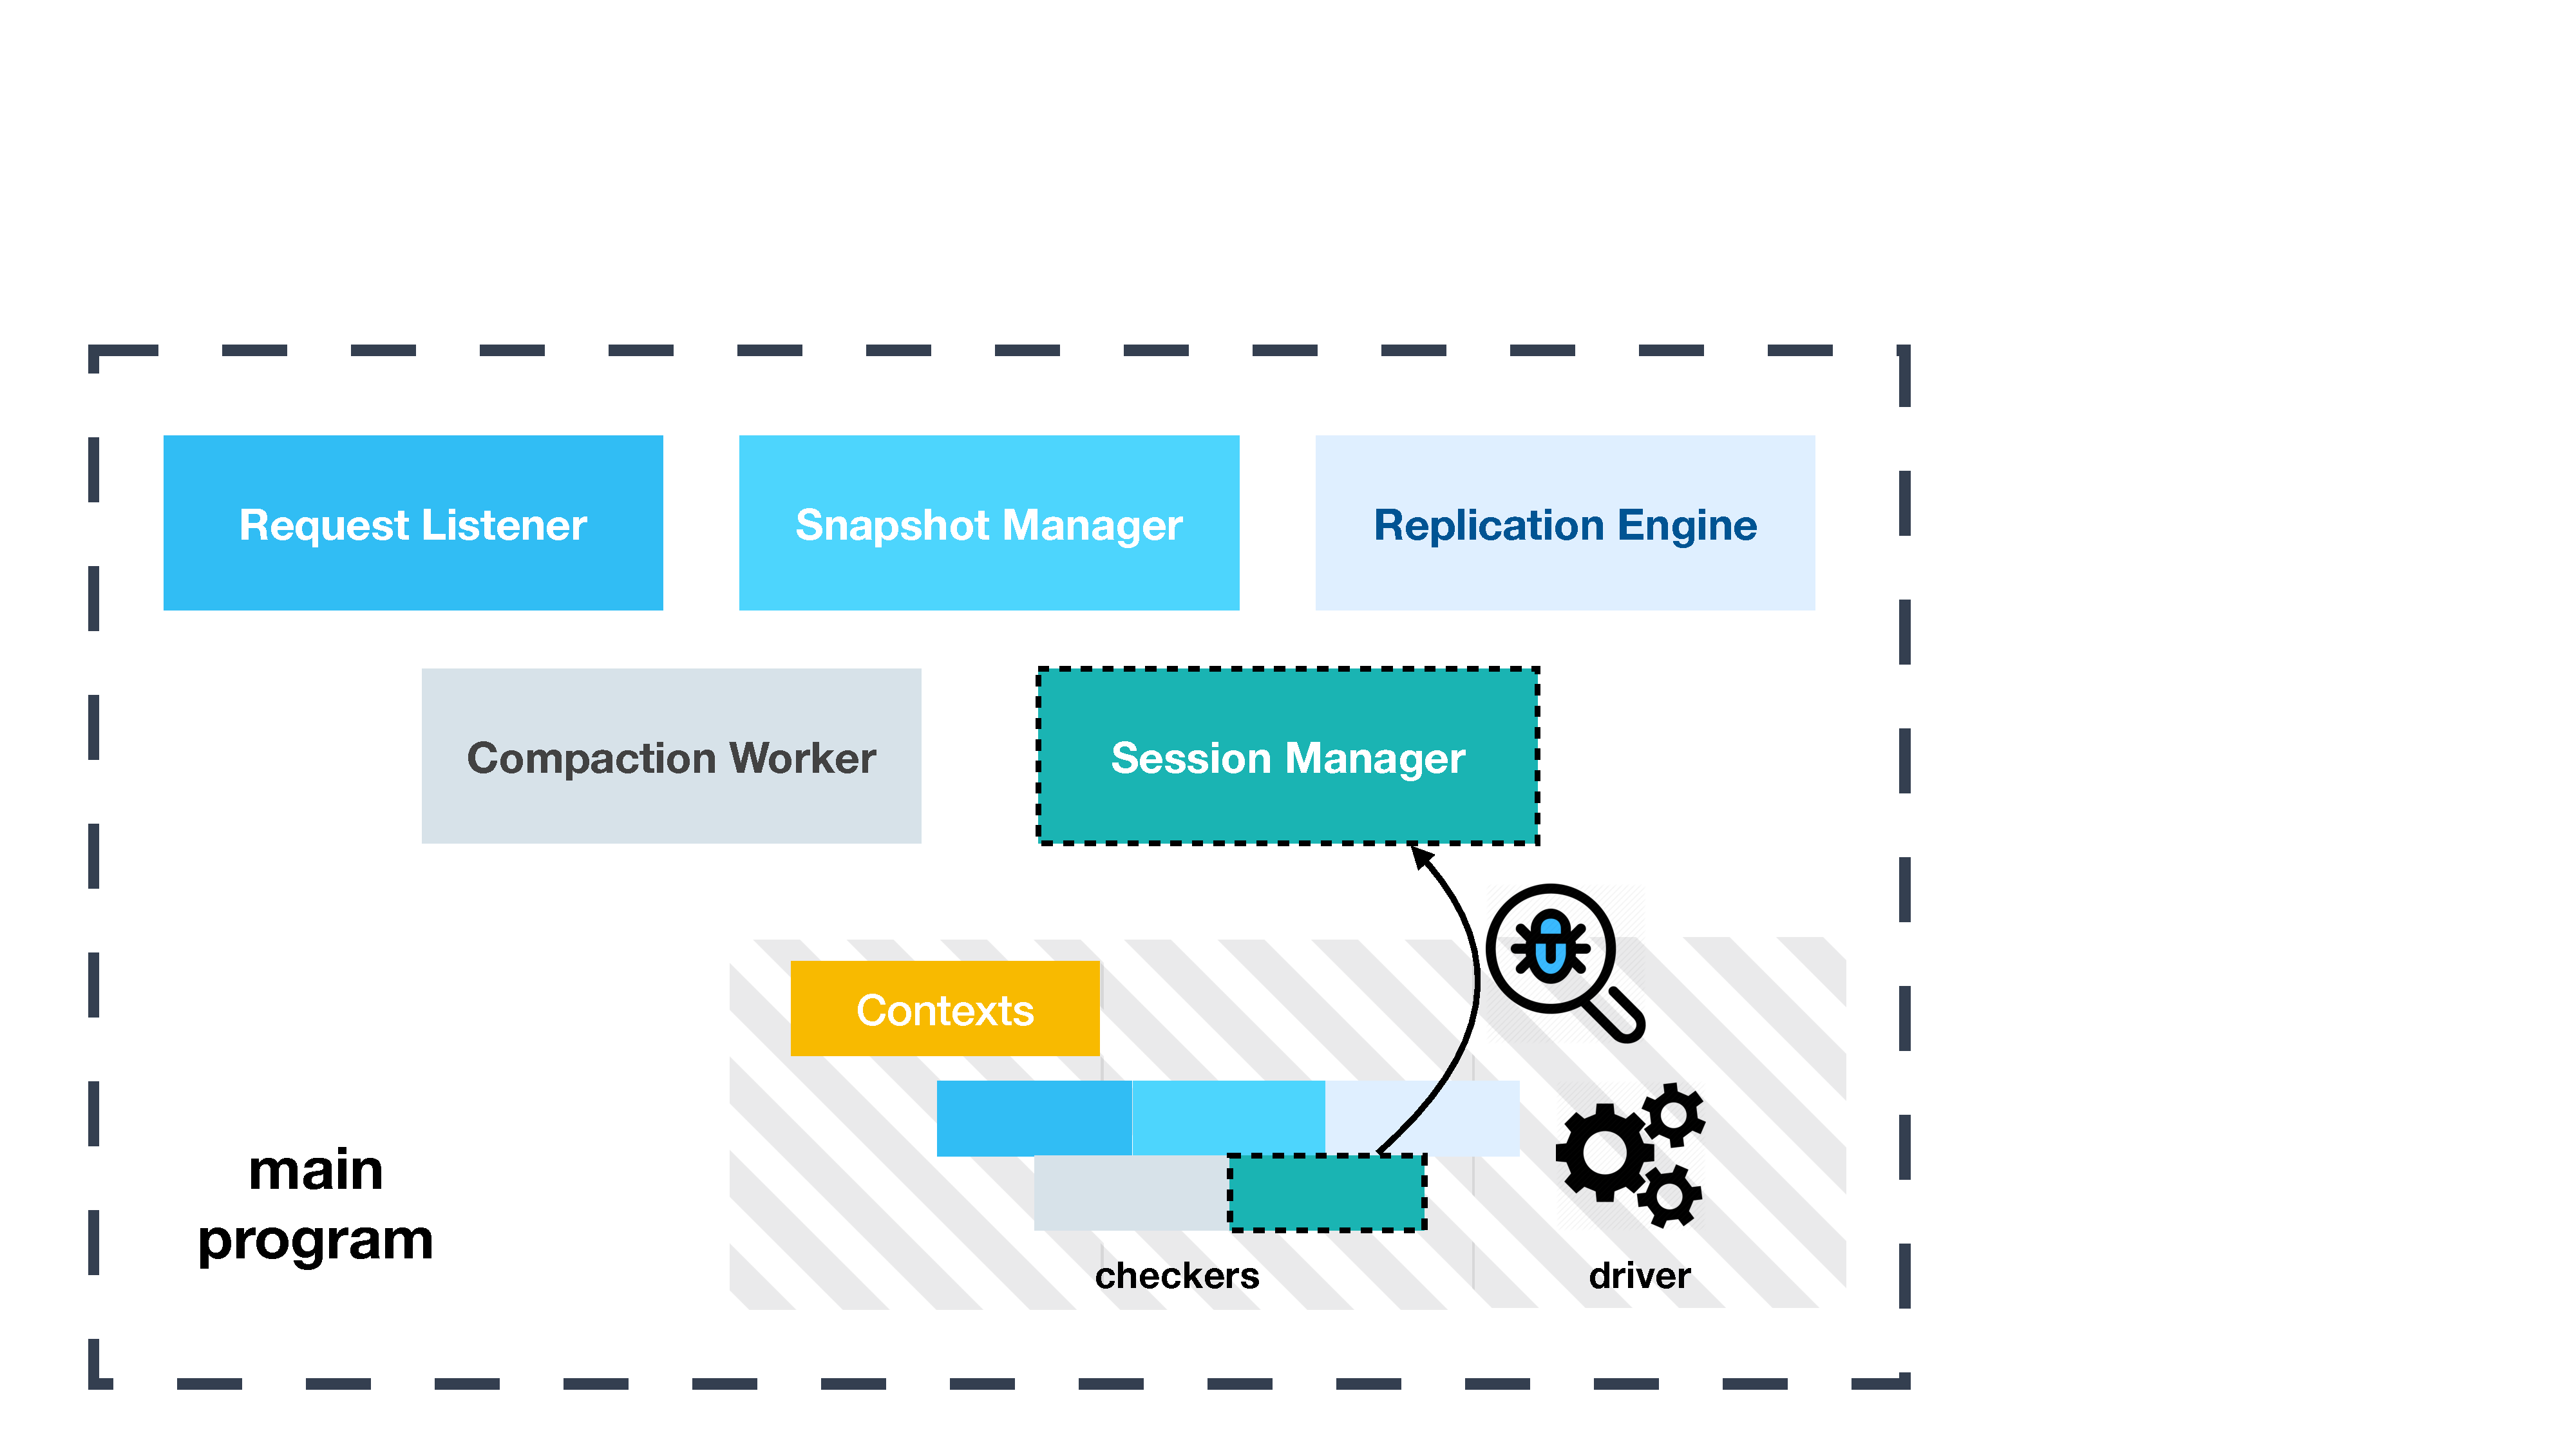
\includegraphics[width=.75\textwidth]{fig/customized}
    \end{center}
\end{frame}

\begin{frame}{Characteristic II: Stateful}
\begin{columns}
    
    \begin{column}{.5\textwidth}
        To synchronized states, introduce
        \begin{block}{\textbf{Context}}
            \begin{itemize}
                \item bound
                to each checker
                \item  holds all the arguments needed for the
                checker execution
                \item  synchronized with the program state through hooks in the main program
                \item update with current state when hooks reached 
            \end{itemize}
        \end{block}
    \end{column}

    \begin{column}{.5\textwidth}

        \begin{center}
            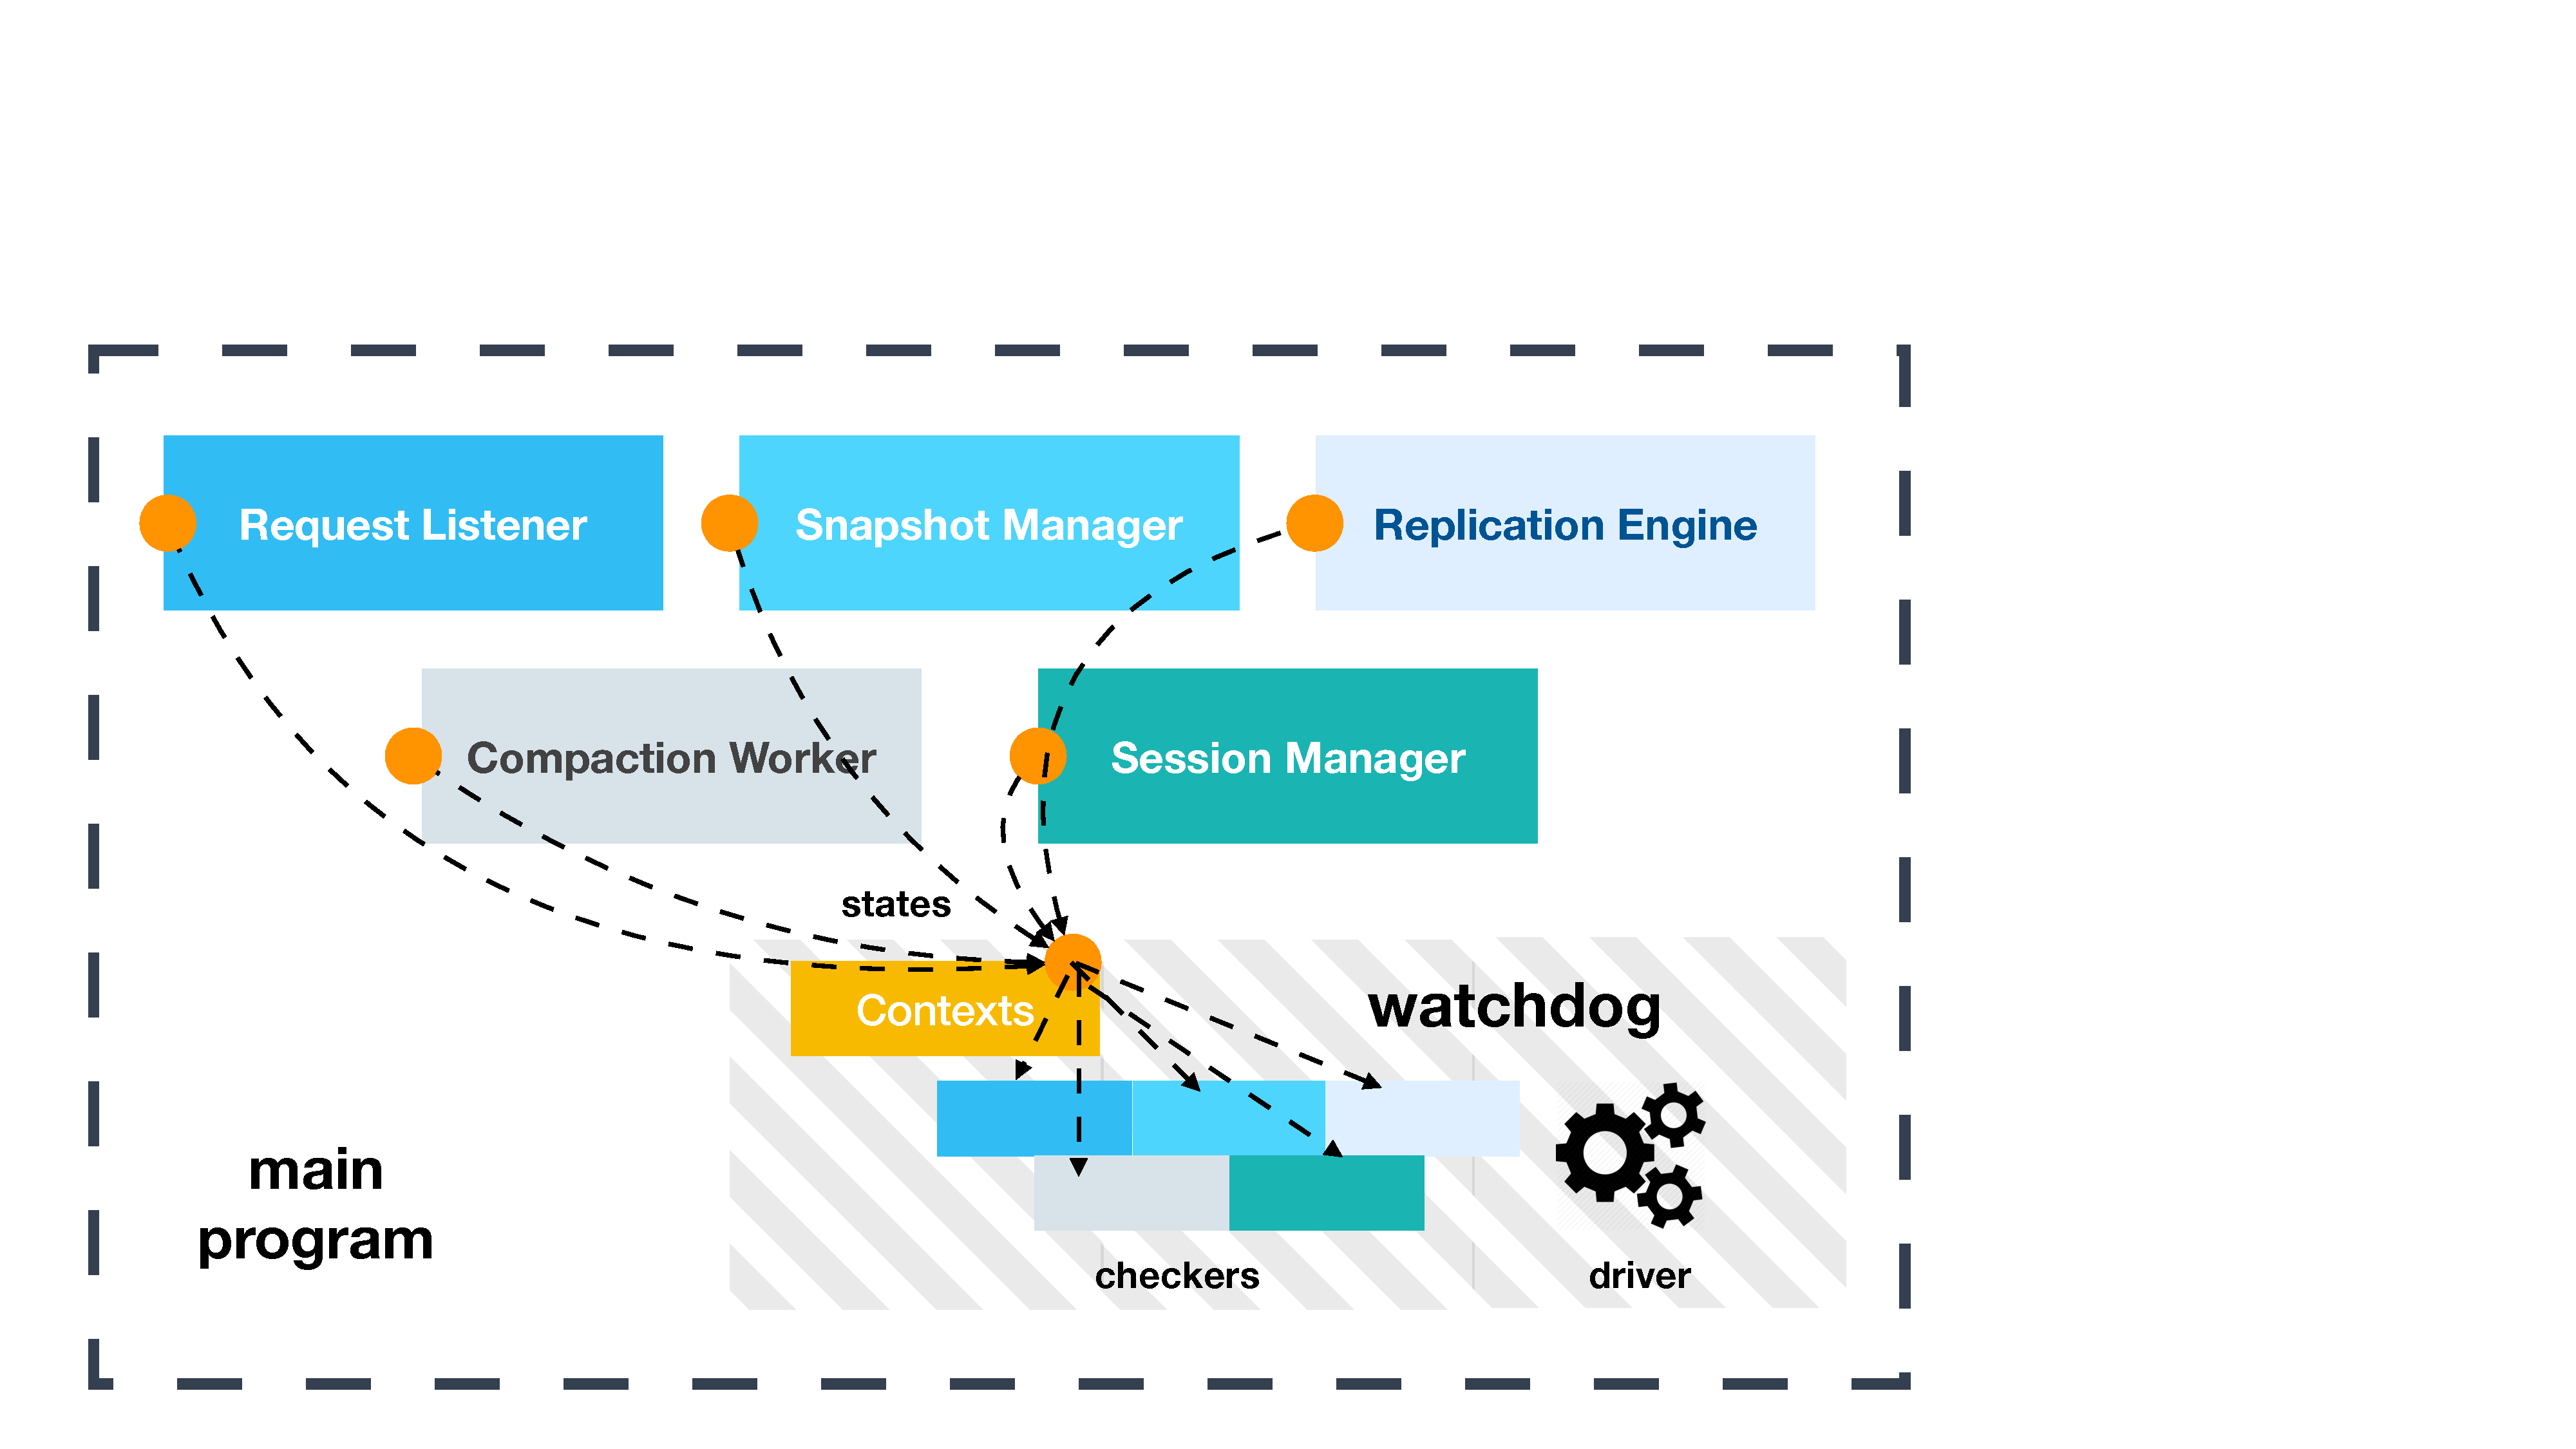
\includegraphics[width=\textwidth]{fig/staetful}
        \end{center}

        \textbf{Note:} The watchdog driver will not execute a checker unless its context is ready.

    \end{column}
\end{columns}

\end{frame}

\begin{frame}{Characteristic III: Concurrent}
    Run watchdog \red{concurrently} with the main program instead of \blue{in-place} checking with \blue{inserted} checkers
    \begin{center}
        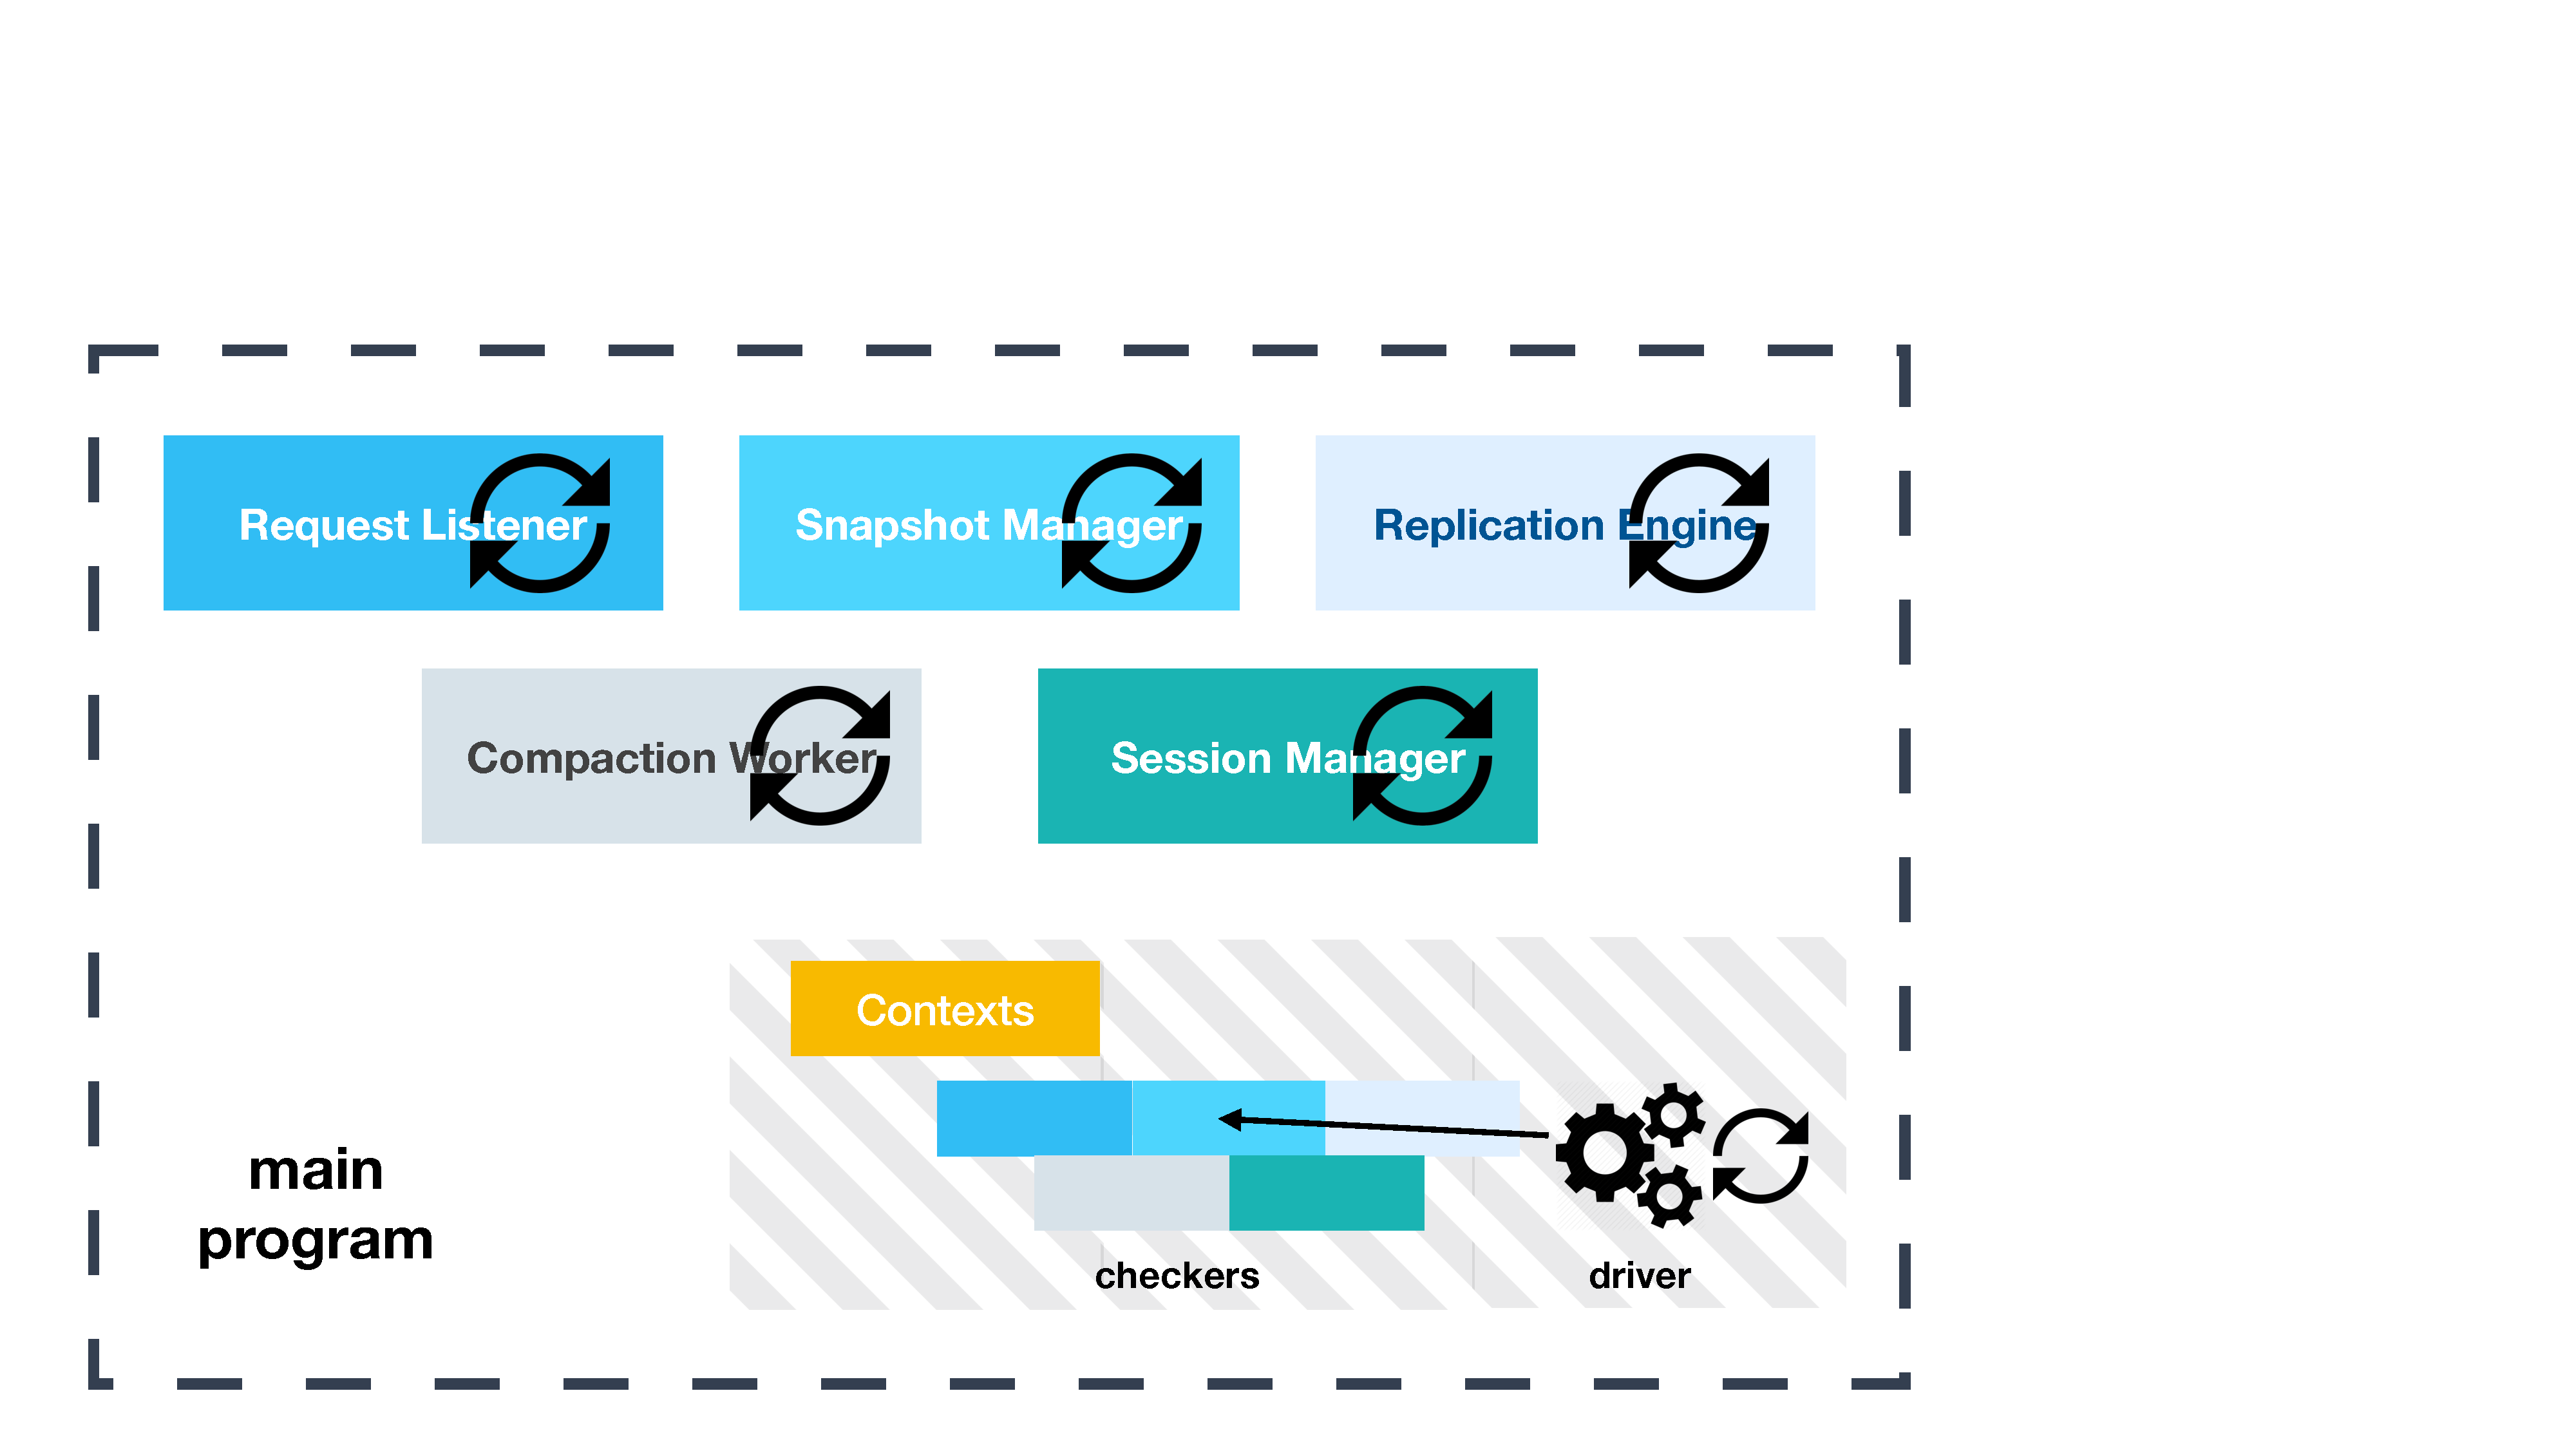
\includegraphics[width=.75
        \textwidth]{fig/concurrent}
    \end{center}
\end{frame}

\begin{frame}{Core Idea: Mimic Checking}
    \begin{center}
        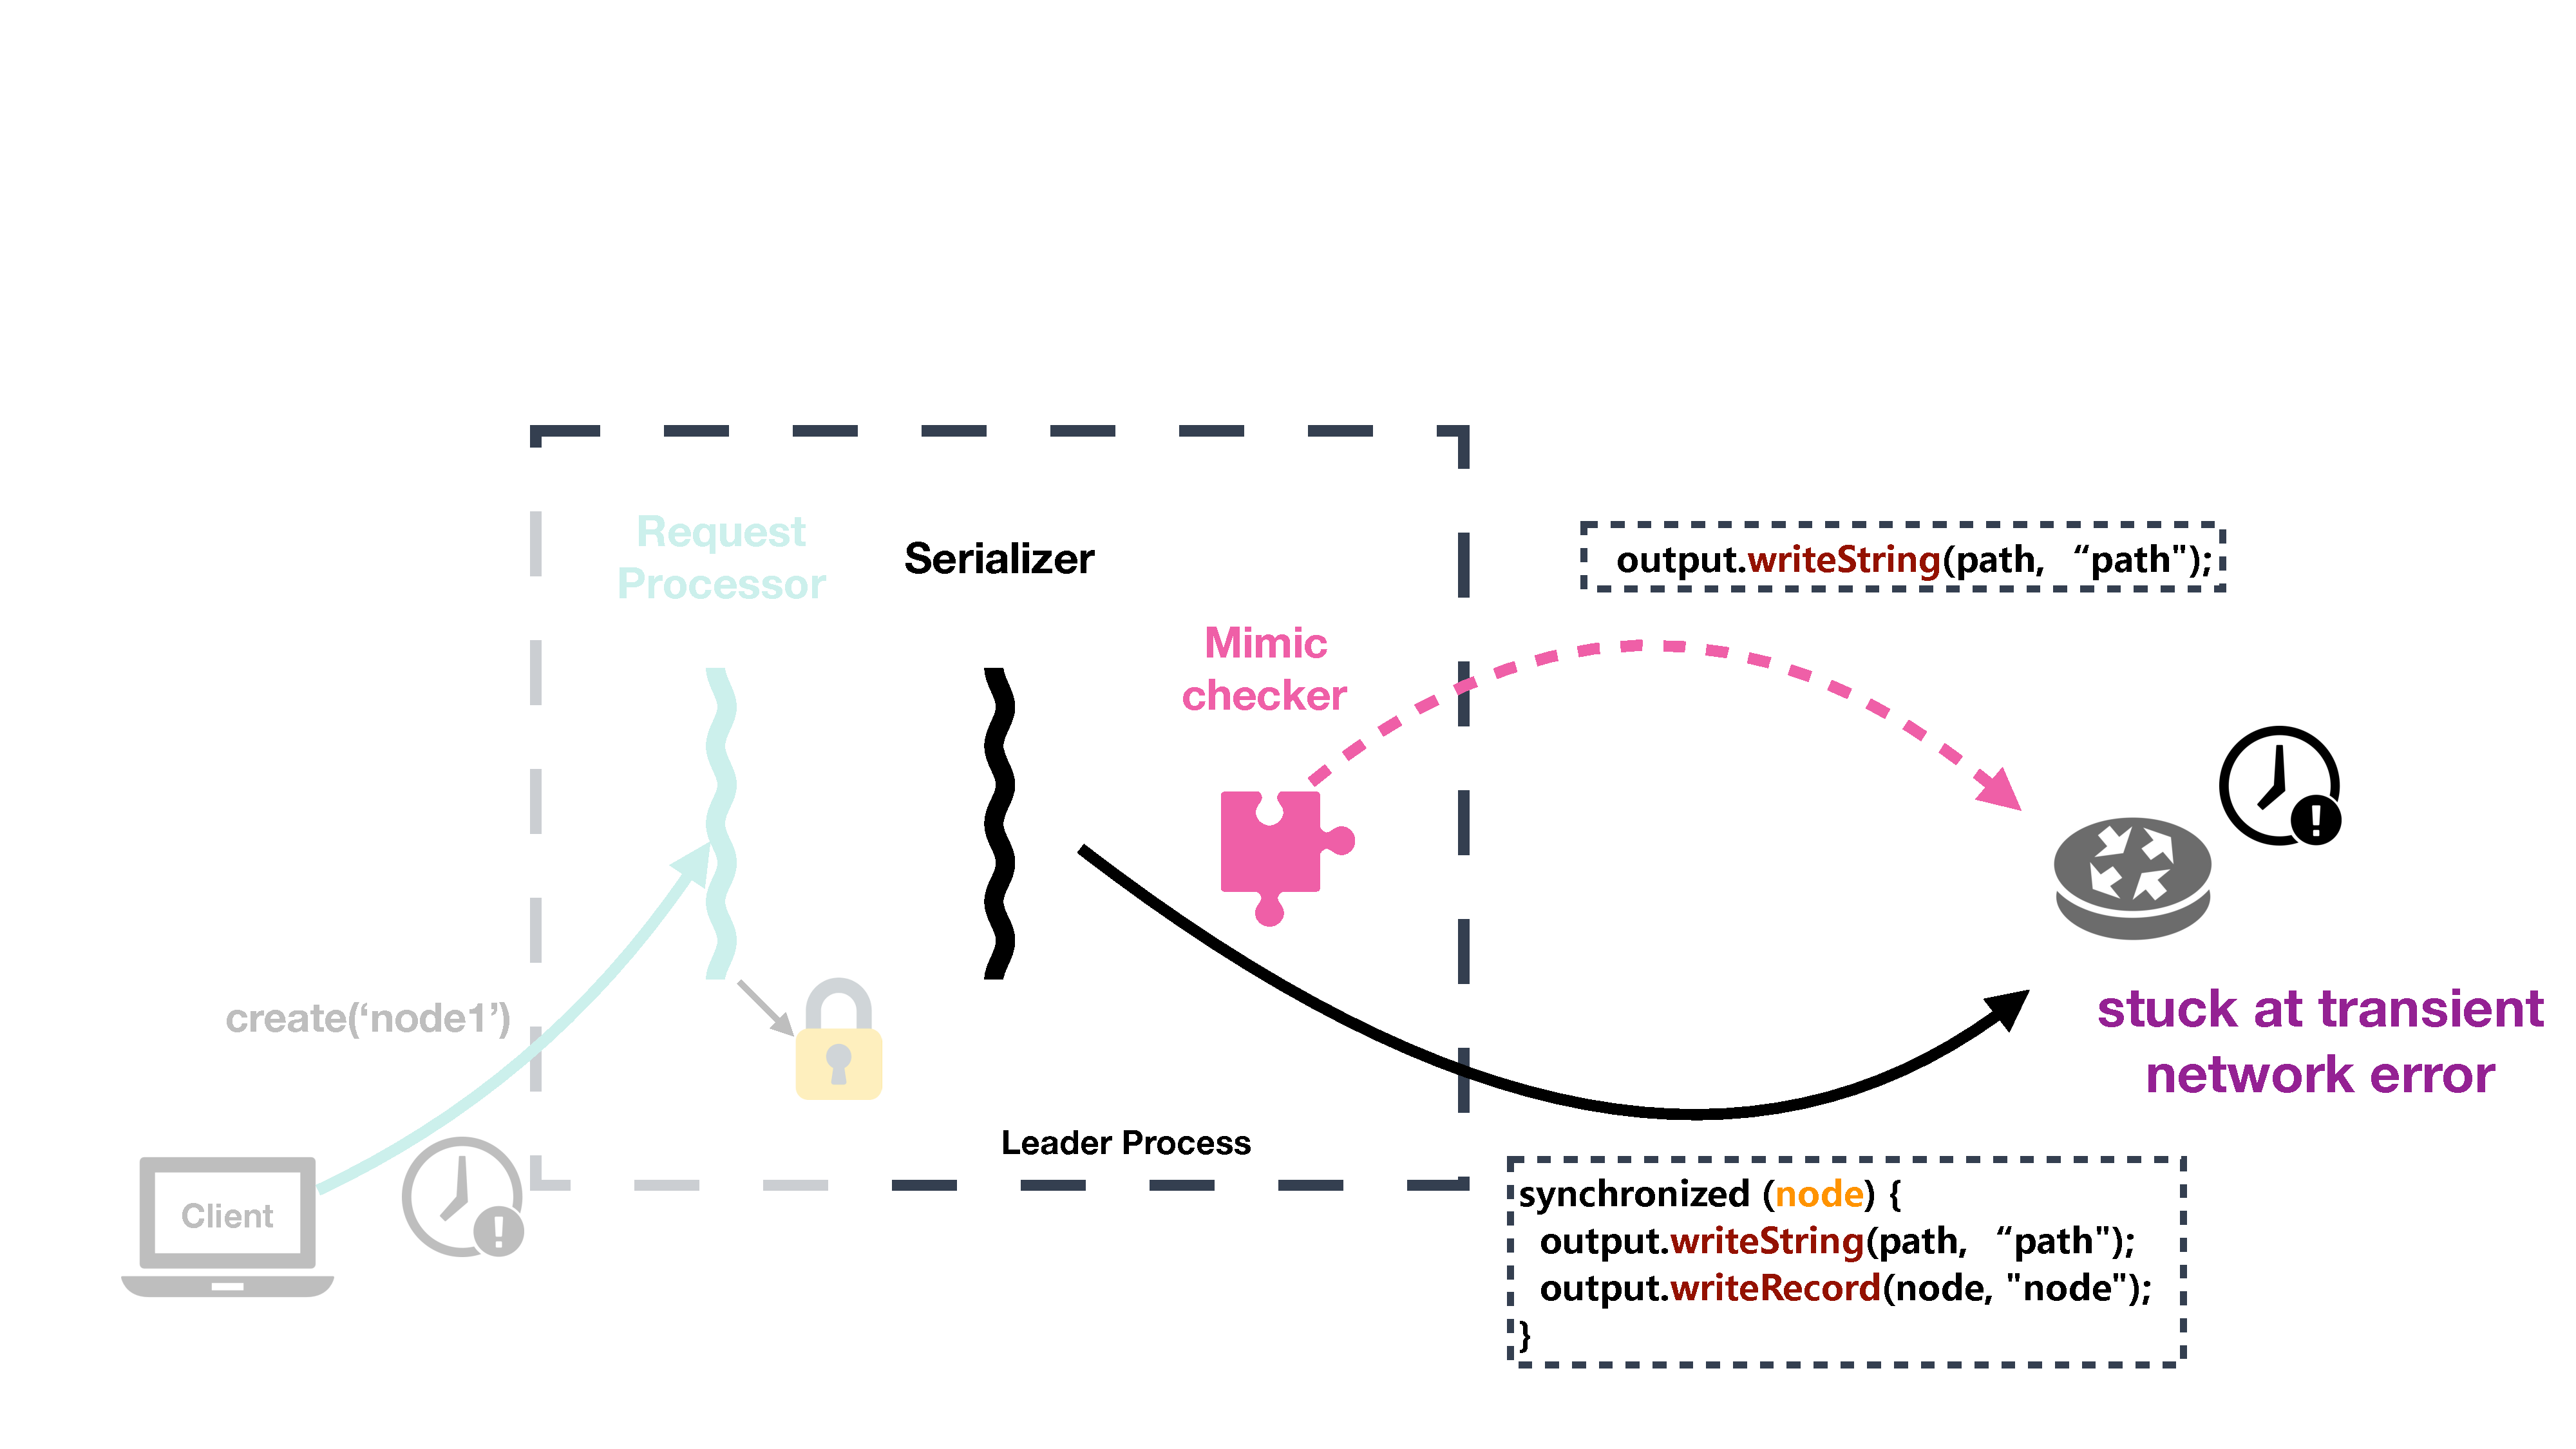
\includegraphics[width=.75\textwidth]{fig/mimic}
    \end{center}
\end{frame}

\end{document}